%# -*- coding: utf-8-unix -*-
%%==================================================
%% thesis.tex
%%==================================================

% 双面打印
% \documentclass[doctor, fontset=adobe, openright, twoside, zihao=-4]{sjtuthesis}
\documentclass[bachelor, fontset=adobe, openany, oneside, zihao=5, submit]{sjtuthesis} 
% \documentclass[master, adobefonts, review]{sjtuthesis} 
% \documentclass[%
%   bachelor|master|doctor,	% 必选项
%   fontset=adobe|windows,  	% 只测试了adobe
%   oneside|twoside,		% 单面打印,双面打印(奇偶页交换页边距,默认)
%   openany|openright, 		% 可以在奇数或者偶数页开新章|只在奇数页开新章(默认)
%   zihao=-4|5,, 		% 正文字号:小四、五号(默认)
%   review,	 		% 盲审论文,隐去作者姓名、学号、导师姓名、致谢、发表论文和参与的项目
%   submit			% 定稿提交的论文,插入签名扫描版的原创性声明、授权声明 
% ]

% 逐个导入参考文献数据库
\addbibresource{bib/thesis.bib}
% \addbibresource{bib/chap2.bib}

\begin{document}

%% 无编号内容:中英文论文封面、授权页
%# -*- coding: utf-8-unix -*-
\title{Android应用崩溃与用户行为分析}
\author{熊\quad{}伟\quad{}伦}
\advisor{戚正伟教授}
\defenddate{2016年6月13日}
\school{上海交通大学}
\institute{电子信息与电气工程学院}
\studentnumber{5120379076}
\major{软件工程}

\englishtitle{Android Application Crash and User Behavior Analysis}
\englishauthor{\textsc{Weilun Xiong}}
\englishadvisor{Prof. \textsc{Zhengwei Qi}}
\englishschool{Shanghai Jiao Tong University}
\englishinstitute{\textsc{School of Electronic Information and Electrical Engineering} \\
  \textsc{Shanghai Jiao Tong University} \\
  \textsc{Shanghai, P.R.China}}
\englishmajor{Software Engineering}
\englishdate{Jun. 13th, 2016}


\maketitle

\makeenglishtitle

\makeatletter
%\ifsjtu@submit\relax
%	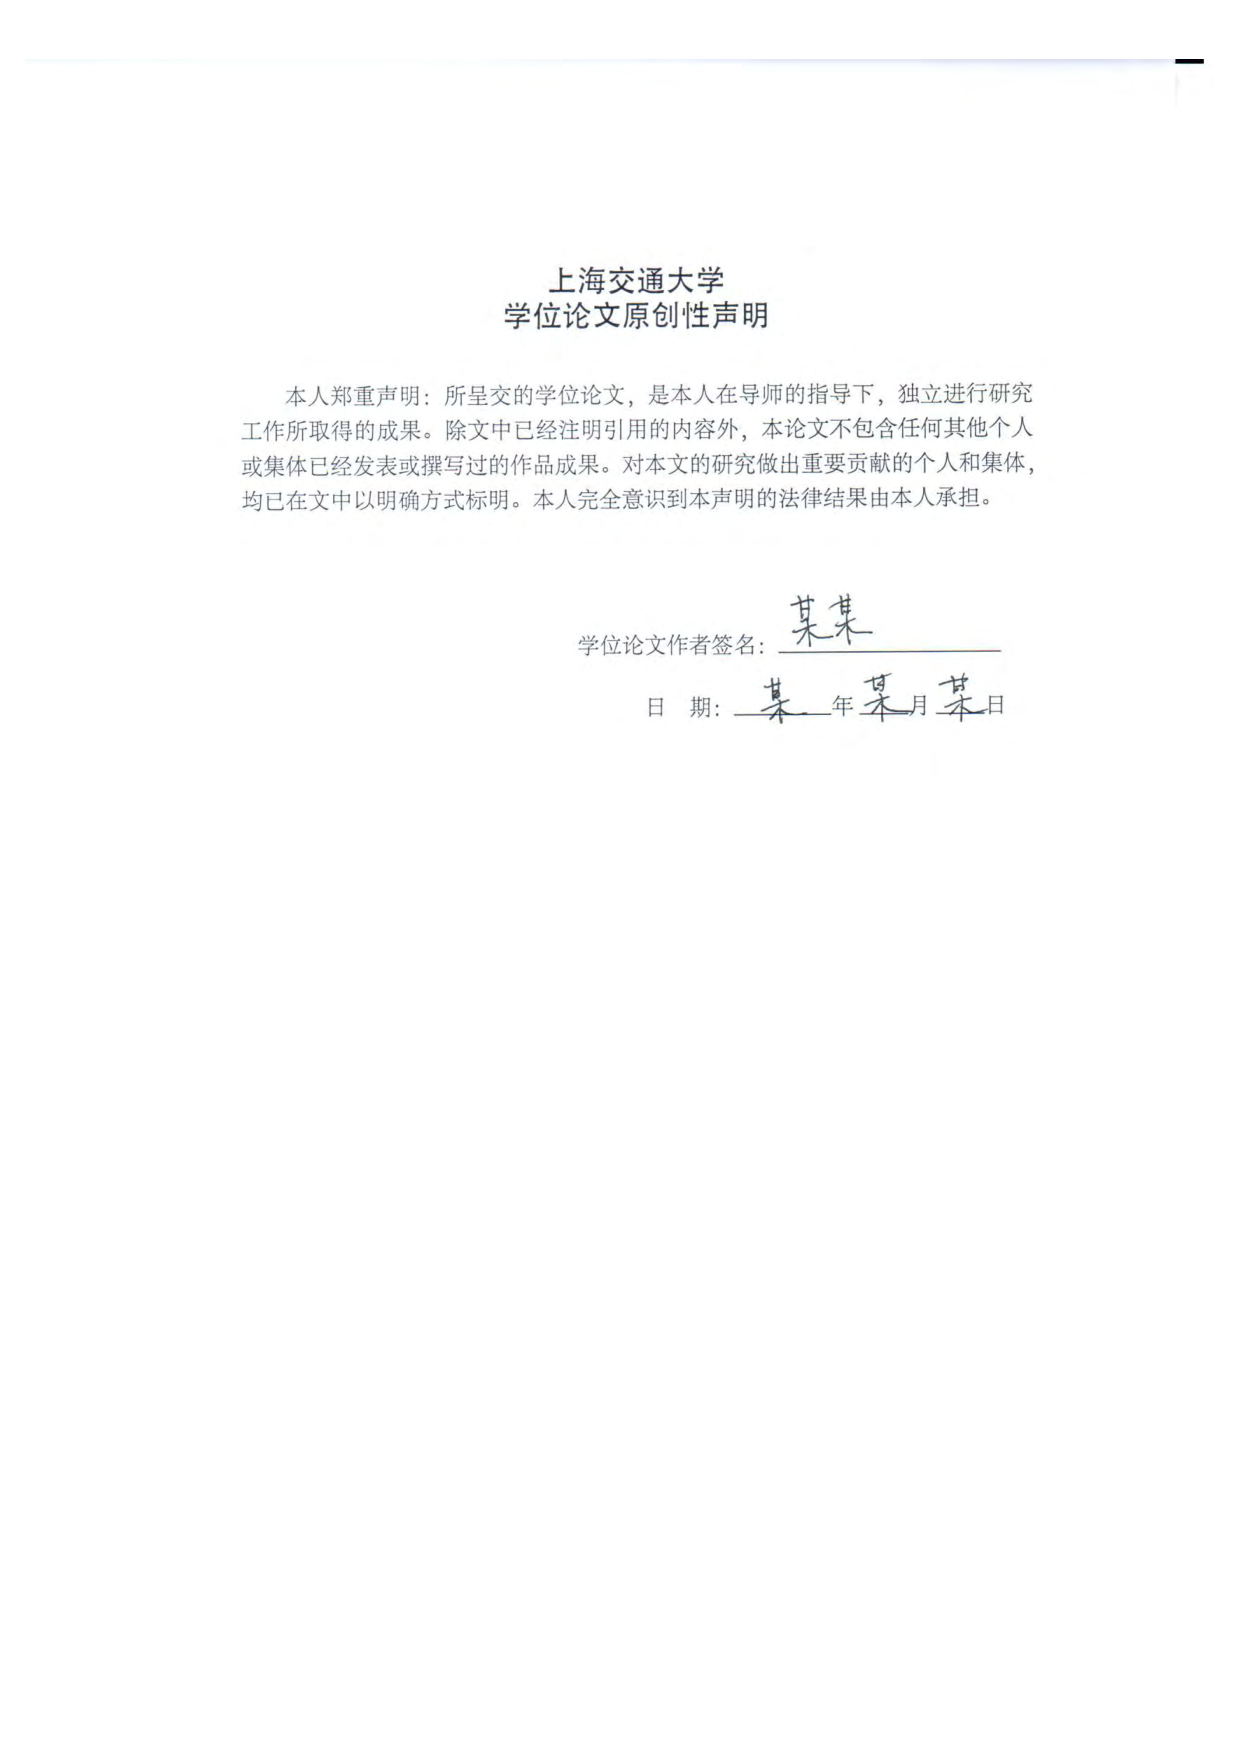
\includepdf{pdf/original.pdf}
%	\cleardoublepage
%	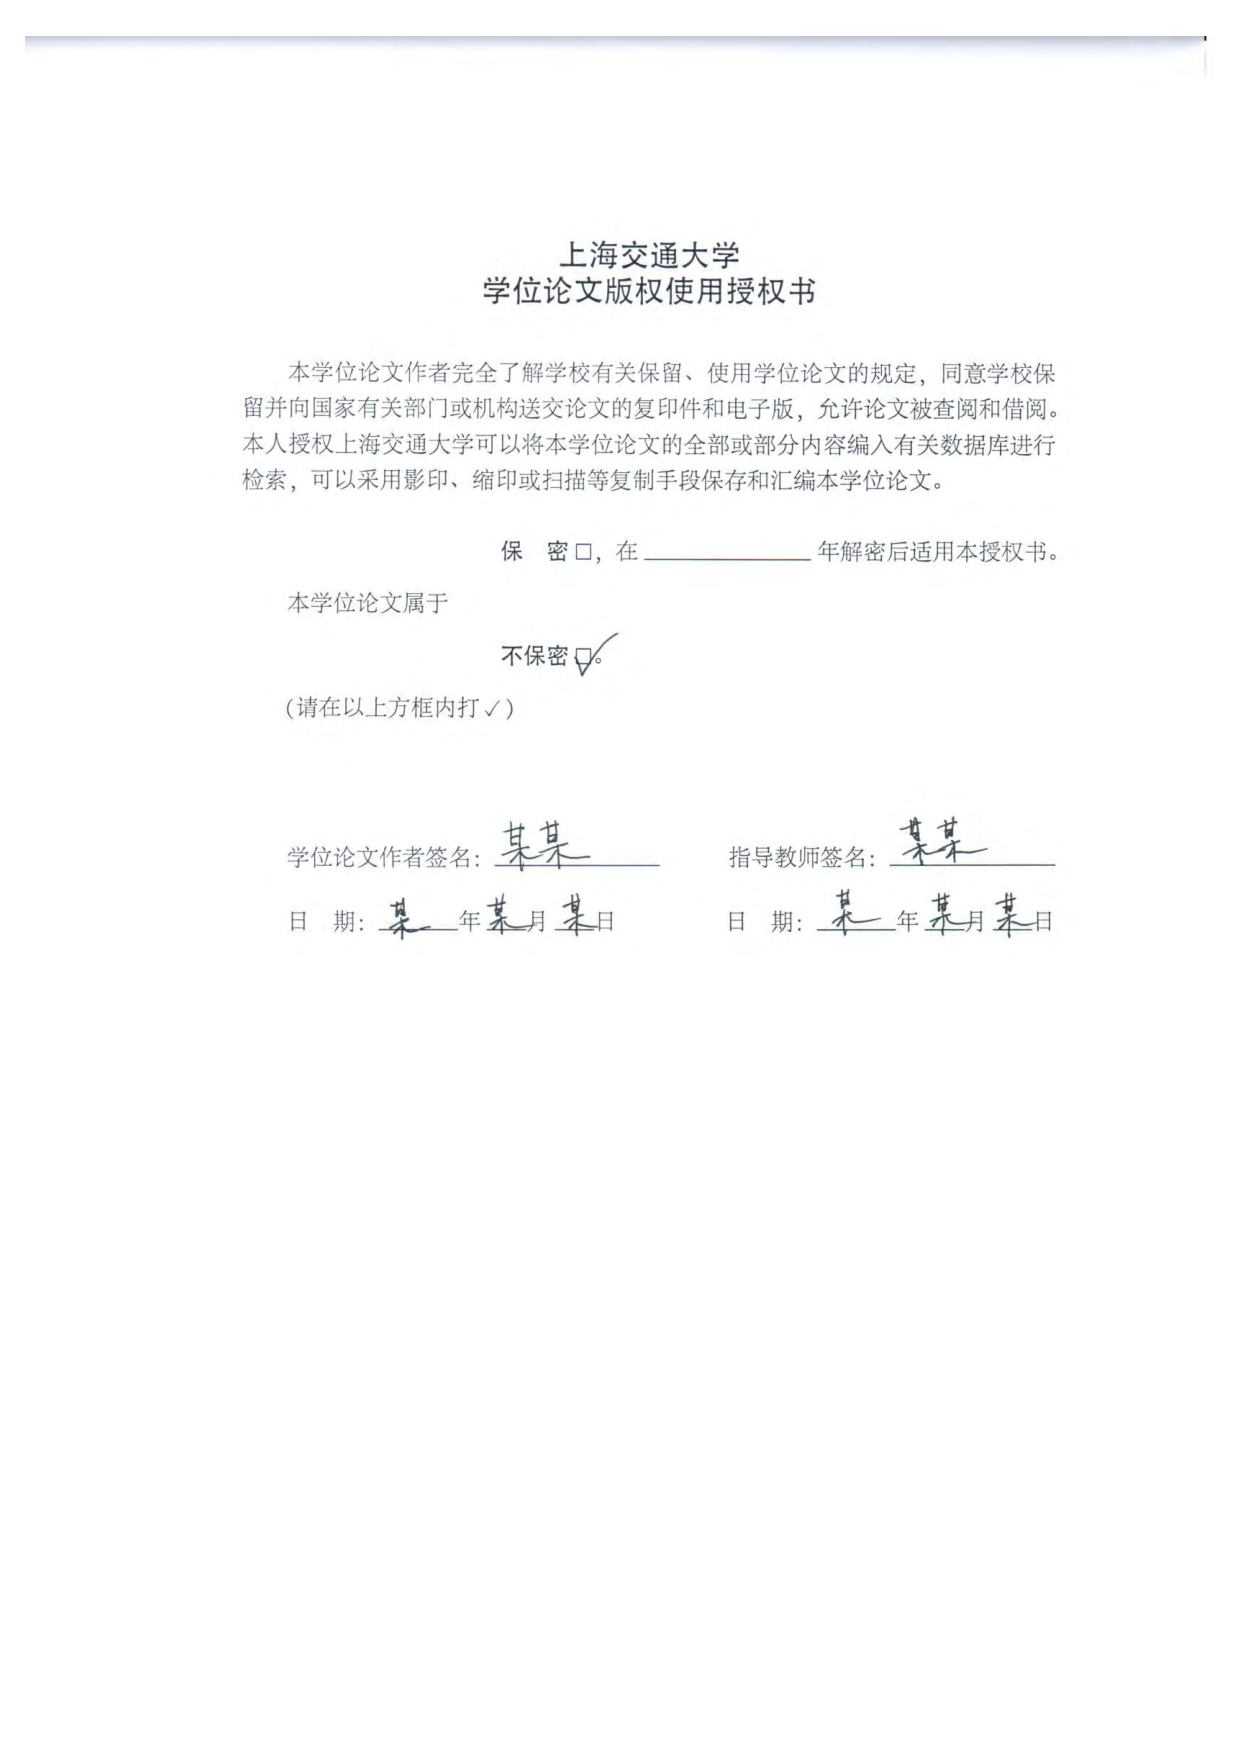
\includepdf{pdf/authorization.pdf}
%	\cleardoublepage
%\else
%	\makeDeclareOriginal
%	\makeDeclareAuthorization
%\fi
\makeatother


\frontmatter 	% 使用罗马数字对前言编号

%% 摘要
\pagestyle{main}
%# -*- coding: utf-8-unix -*-
%%==================================================
%% abstract.tex for SJTU Master Thesis
%%==================================================

\begin{abstract}

上海交通大学是我国历史最悠久的高等学府之一,是教育部直属、教育部与上海市共建的全国重点大学,是国家 “七五”、“八五”重点建设和“211工程”、“985工程”的首批建设高校。经过115年的不懈努力,上海交通大学已经成为一所“综合性、研究型、国际化”的国内一流、国际知名大学,并正在向世界一流大学稳步迈进。 

十九世纪末,甲午战败,民族危难。中国近代著名实业家、教育家盛宣怀和一批有识之士秉持“自强首在储才,储才必先兴学”的信念,于1896年在上海创办了交通大学的前身——南洋公学。建校伊始,学校即坚持“求实学,务实业”的宗旨,以培养“第一等人才”为教育目标,精勤进取,笃行不倦,在二十世纪二三十年代已成为国内著名的高等学府,被誉为“东方MIT”。抗战时期,广大师生历尽艰难,移转租界,内迁重庆,坚持办学,不少学生投笔从戎,浴血沙场。解放前夕,广大师生积极投身民主革命,学校被誉为“民主堡垒”。

新中国成立初期,为配合国家经济建设的需要,学校调整出相当一部分优势专业、师资设备,支持国内兄弟院校的发展。五十年代中期,学校又响应国家建设大西北的号召,根据国务院决定,部分迁往西安,分为交通大学上海部分和西安部分。1959年3月两部分同时被列为全国重点大学,7月经国务院批准分别独立建制,交通大学上海部分启用“上海交通大学”校名。历经西迁、两地办学、独立办学等变迁,为构建新中国的高等教育体系,促进社会主义建设做出了重要贡献。六七十年代,学校先后归属国防科工委和六机部领导,积极投身国防人才培养和国防科研,为“两弹一星”和国防现代化做出了巨大贡献。

改革开放以来,学校以“敢为天下先”的精神,大胆推进改革:率先组成教授代表团访问美国,率先实行校内管理体制改革,率先接受海外友人巨资捐赠等,有力地推动了学校的教学科研改革。1984年,邓小平同志亲切接见了学校领导和师生代表,对学校的各项改革给予了充分肯定。在国家和上海市的大力支持下,学校以“上水平、创一流”为目标,以学科建设为龙头,先后恢复和兴建了理科、管理学科、生命学科、法学和人文学科等。1999年,上海农学院并入;2005年,与上海第二医科大学强强合并。至此,学校完成了综合性大学的学科布局。近年来,通过国家“985工程”和“211工程”的建设,学校高层次人才日渐汇聚,科研实力快速提升,实现了向研究型大学的转变。与此同时,学校通过与美国密西根大学等世界一流大学的合作办学,实施国际化战略取得重要突破。1985年开始闵行校区建设,历经20多年,已基本建设成设施完善,环境优美的现代化大学校园,并已完成了办学重心向闵行校区的转移。学校现有徐汇、闵行、法华、七宝和重庆南路(卢湾)5个校区,总占地面积4840亩。通过一系列的改革和建设,学校的各项办学指标大幅度上升,实现了跨越式发展,整体实力显著增强,为建设世界一流大学奠定了坚实的基础。

交通大学始终把人才培养作为办学的根本任务。一百多年来,学校为国家和社会培养了20余万各类优秀人才,包括一批杰出的政治家、科学家、社会活动家、实业家、工程技术专家和医学专家,如江泽民、陆定一、丁关根、汪道涵、钱学森、吴文俊、徐光宪、张光斗、黄炎培、邵力子、李叔同、蔡锷、邹韬奋、陈敏章、王振义、陈竺等。在中国科学院、中国工程院院士中,有200余位交大校友;在国家23位“两弹一星”功臣中,有6位交大校友;在18位国家最高科学技术奖获得者中,有3位来自交大。交大创造了中国近现代发展史上的诸多“第一”:中国最早的内燃机、最早的电机、最早的中文打字机等;新中国第一艘万吨轮、第一艘核潜艇、第一艘气垫船、第一艘水翼艇、自主设计的第一代战斗机、第一枚运载火箭、第一颗人造卫星、第一例心脏二尖瓣分离术、第一例成功移植同种原位肝手术、第一例成功抢救大面积烧伤病人手术等,都凝聚着交大师生和校友的心血智慧。改革开放以来,一批年轻的校友已在世界各地、各行各业崭露头角。

截至2011年12月31日,学校共有24个学院/直属系(另有继续教育学院、技术学院和国际教育学院),19个直属单位,12家附属医院,全日制本科生16802人、研究生24495人(其中博士研究生5059人);有专任教师2979名,其中教授835名;中国科学院院士15名,中国工程院院士20名,中组部“千人计划”49名,“长江学者”95名,国家杰出青年基金获得者80名,国家重点基础研究发展计划(973计划)首席科学家24名,国家重大科学研究计划首席科学家9名,国家基金委创新研究群体6个,教育部创新团队17个。

学校现有本科专业68个,涵盖经济学、法学、文学、理学、工学、农学、医学、管理学和艺术等九个学科门类;拥有国家级教学及人才培养基地7个,国家级校外实践教育基地5个,国家级实验教学示范中心5个,上海市实验教学示范中心4个;有国家级教学团队8个,上海市教学团队15个;有国家级教学名师7人,上海市教学名师35人;有国家级精品课程46门,上海市精品课程117门;有国家级双语示范课程7门;2001、2005和2009年,作为第一完成单位,共获得国家级教学成果37项、上海市教学成果157项。

\keywords{\large 上海交大 \quad 饮水思源 \quad 爱国荣校}
\end{abstract}

\begin{englishabstract}

An imperial edict issued in 1896 by Emperor Guangxu, established Nanyang Public School in Shanghai. The normal school, school of foreign studies, middle school and a high school were established. Sheng Xuanhuai, the person responsible for proposing the idea to the emperor, became the first president and is regarded as the founder of the university.

During the 1930s, the university gained a reputation of nurturing top engineers. After the foundation of People's Republic, some faculties were transferred to other universities. A significant amount of its faculty were sent in 1956, by the national government, to Xi'an to help build up Xi'an Jiao Tong University in western China. Afterwards, the school was officially renamed Shanghai Jiao Tong University.

Since the reform and opening up policy in China, SJTU has taken the lead in management reform of institutions for higher education, regaining its vigor and vitality with an unprecedented momentum of growth. SJTU includes five beautiful campuses, Xuhui, Minhang, Luwan Qibao, and Fahua, taking up an area of about 3,225,833 m2. A number of disciplines have been advancing towards the top echelon internationally, and a batch of burgeoning branches of learning have taken an important position domestically.

Today SJTU has 31 schools (departments), 63 undergraduate programs, 250 masters-degree programs, 203 Ph.D. programs, 28 post-doctorate programs, and 11 state key laboratories and national engineering research centers.

SJTU boasts a large number of famous scientists and professors, including 35 academics of the Academy of Sciences and Academy of Engineering, 95 accredited professors and chair professors of the "Cheung Kong Scholars Program" and more than 2,000 professors and associate professors.

Its total enrollment of students amounts to 35,929, of which 1,564 are international students. There are 16,802 undergraduates, and 17,563 masters and Ph.D. candidates. After more than a century of operation, Jiao Tong University has inherited the old tradition of "high starting points, solid foundation, strict requirements and extensive practice." Students from SJTU have won top prizes in various competitions, including ACM International Collegiate Programming Contest, International Mathematical Contest in Modeling and Electronics Design Contests. Famous alumni include Jiang Zemin, Lu Dingyi, Ding Guangen, Wang Daohan, Qian Xuesen, Wu Wenjun, Zou Taofen, Mao Yisheng, Cai Er, Huang Yanpei, Shao Lizi, Wang An and many more. More than 200 of the academics of the Chinese Academy of Sciences and Chinese Academy of Engineering are alumni of Jiao Tong University.

\englishkeywords{\large SJTU, master thesis, XeTeX/LaTeX template}
\end{englishabstract}



%% 目录、插图目录、表格目录
\tableofcontents
% \listoffigures
% \addcontentsline{toc}{chapter}{\listfigurename} %将插图目录加入全文目录
% \listoftables
% \addcontentsline{toc}{chapter}{\listtablename}  %将表格目录加入全文目录
% \listofalgorithms
% \addcontentsline{toc}{chapter}{算法索引}        %将算法目录加入全文目录

% %# -*- coding: utf-8-unix -*-
\chapter{主要符号对照表}
\label{chap:symb}

\begin{longtable}{rl}
$\epsilon$     & 介电常数 \\
 $\mu$ 		& 磁导率 \\
 $\epsilon$     & 介电常数 \\
 $\mu$ 		& 磁导率 \\
 $\epsilon$     & 介电常数 \\
 $\mu$ 		& 磁导率 \\
 $\epsilon$ 	& 介电常数 \\
 $\mu$ 		& 磁导率 \\
 $\epsilon$     & 介电常数 \\
 $\mu$ 		& 磁导率 \\
 $\epsilon$     & 介电常数 \\
 $\mu$ 		& 磁导率 \\
 $\epsilon$     & 介电常数 \\
 $\mu$ 		& 磁导率 \\
 $\epsilon$ 	& 介电常数 \\
 $\mu$ 		& 磁导率 \\
 $\epsilon$     & 介电常数 \\
 $\mu$ 		& 磁导率 \\
 $\epsilon$     & 介电常数 \\
 $\mu$ 		& 磁导率 \\
 $\epsilon$     & 介电常数 \\
 $\mu$ 		& 磁导率 \\
 $\epsilon$ 	& 介电常数 \\
 $\mu$ 		& 磁导率 \\
 $\epsilon$     & 介电常数 \\
 $\mu$ 		& 磁导率 \\
 $\epsilon$     & 介电常数 \\
 $\mu$ 		& 磁导率 \\
 $\epsilon$     & 介电常数 \\
 $\mu$ 		& 磁导率 \\
 $\epsilon$ 	& 介电常数 \\
 $\mu$ 		& 磁导率 \\
 $\epsilon$     & 介电常数 \\
 $\mu$ 		& 磁导率 \\
 $\epsilon$     & 介电常数 \\
 $\mu$ 		& 磁导率 \\
 $\epsilon$     & 介电常数 \\
 $\mu$ 		& 磁导率 \\
 $\epsilon$ 	& 介电常数 \\
 $\mu$ 		& 磁导率 \\
 $\epsilon$     & 介电常数 \\
 $\mu$ 		& 磁导率 \\
 $\epsilon$     & 介电常数 \\
 $\mu$ 		& 磁导率 \\
 $\epsilon$     & 介电常数 \\
 $\mu$ 		& 磁导率 \\
 $\epsilon$ 	& 介电常数 \\
 $\mu$ 		& 磁导率 \\
 $\epsilon$     & 介电常数 \\
 $\mu$ 		& 磁导率 \\
 $\epsilon$     & 介电常数 \\
 $\mu$ 		& 磁导率 \\
 $\epsilon$     & 介电常数 \\
 $\mu$ 		& 磁导率 \\
\end{longtable}
 % 主要符号、缩略词对照表

\mainmatter	% 使用阿拉伯数字对正文编号

%% 正文内容
\pagestyle{main}
%# -*- coding: utf-8-unix -*-

%\bibliographystyle{sjtu2}%[此处用于每章都生产参考文献]
\chapter{绪论}
\label{chap:intro}

运行Android系统的设备数量随着移动互联网的兴起爆发式增长,2014年著名的视频网站YouTube超过一半的流量来自于移动设备[1]。

根据Google公司的统计,截止2015年9月30日,在全球范围内已激活的Android设备已经达到14亿台[2],超过微软公司的Windows,苹果公司的OS X和iOS,是全球运行设备数量最多的商用操作系统。

\section{Android生态系统}
\label{sec:android_ecosystem}

通常每台智能手机运行着数十至上百个应用程序,简称App。
其中一部分是制造设备的厂商或定制Android操作系统厂商的App,但用户每天接触时间最长的是第三方的应用厂商或者独立开发者开发的,并且需要连接互联网的App。

在Android生态系统中,开发者完成Android App的开发完后,需要通过诸如Google Play Store、腾讯应用宝、小米应用商店等Android应用市场发布App,应用市场会对开发者提交的App进行安全、内容和程序稳定性上的审核,通过审核后,用户再从应用市场搜索App进行下载安装和使用,流程如图\ref{fig:IndustryChain}所示。
%TODO 引用艾媒咨询

\begin{figure}[!htp]
	\centering
	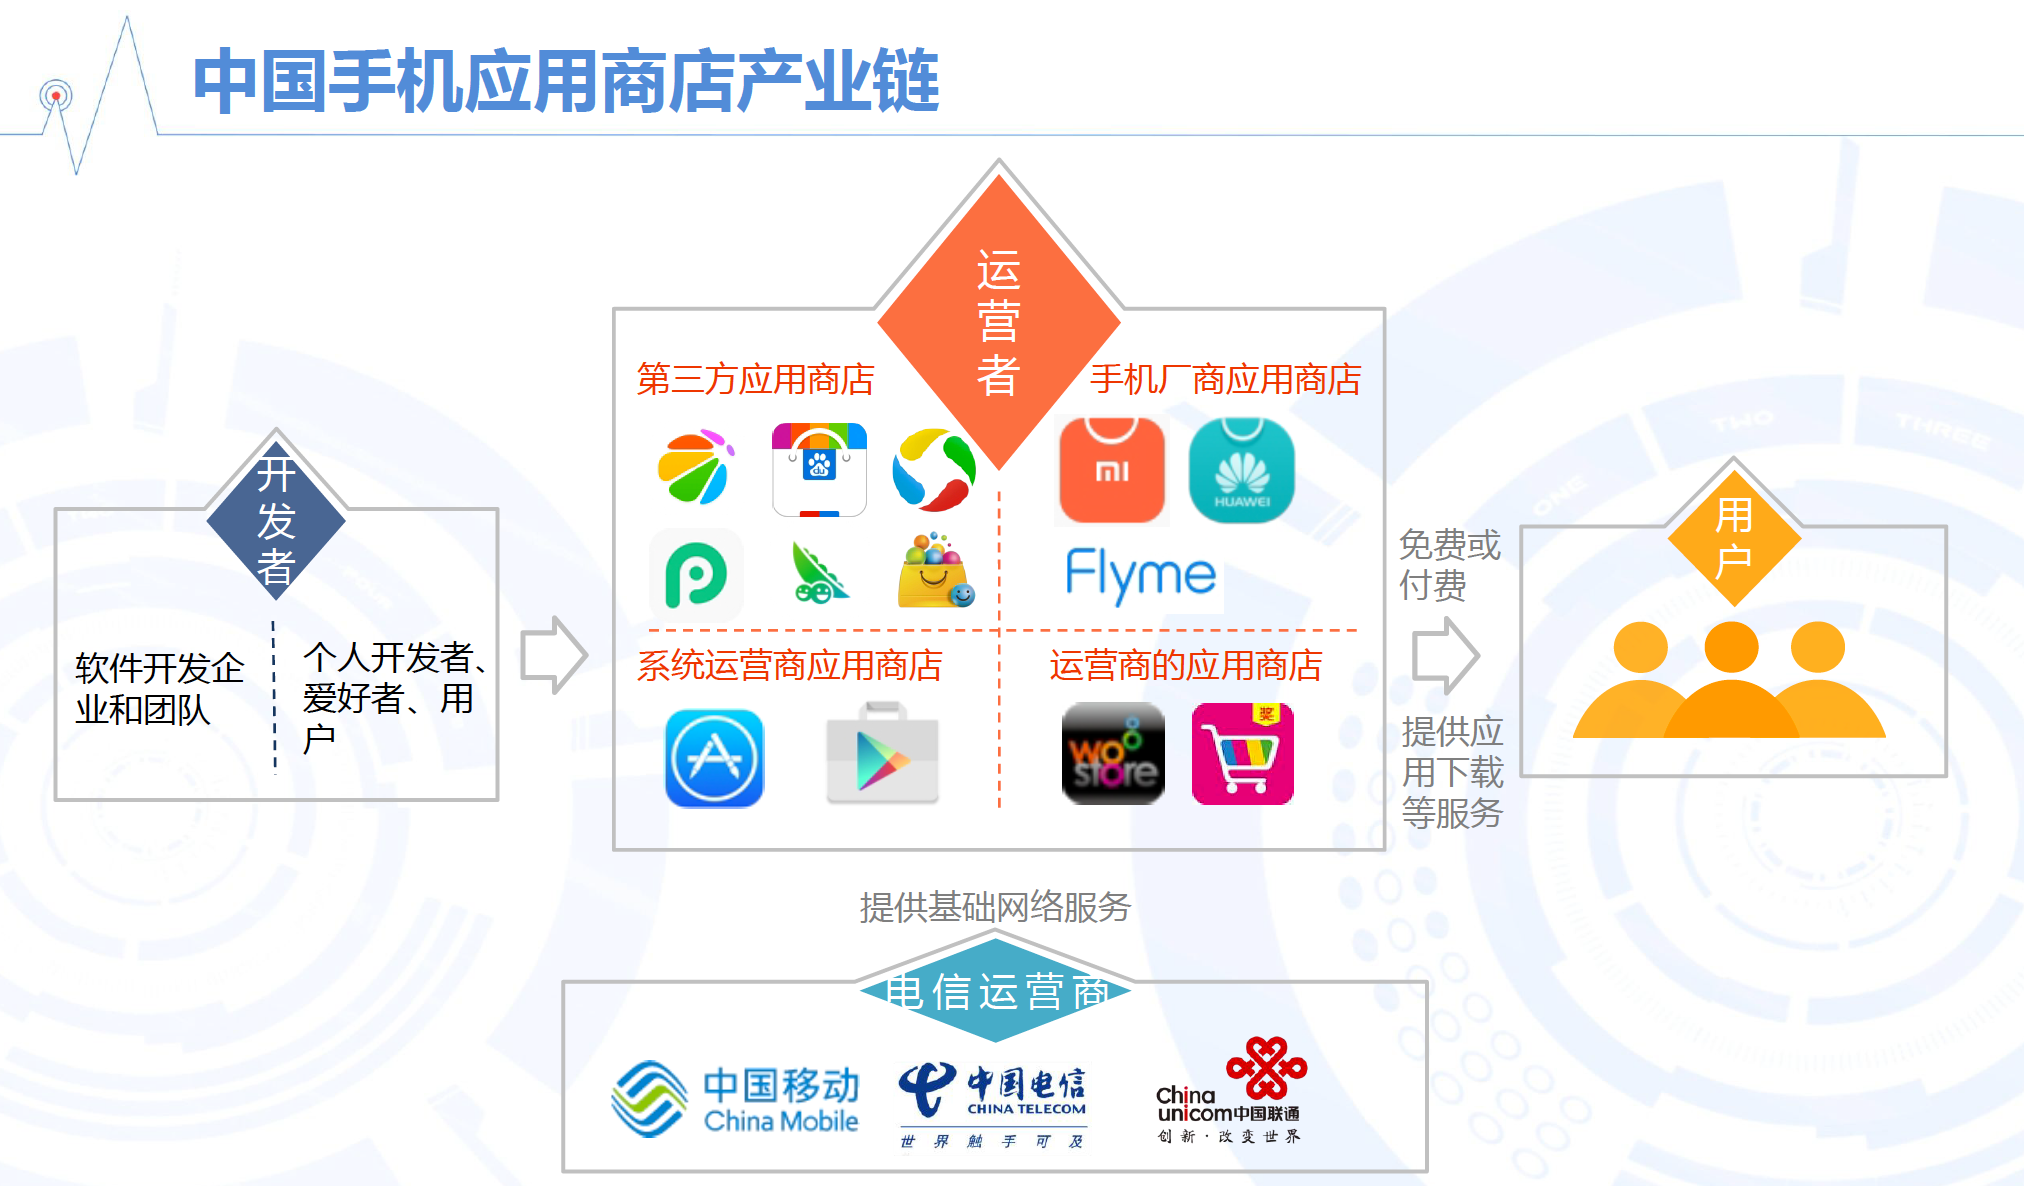
\includegraphics[width=1\textwidth]{industry_chain.png}
	\bicaption[fig:IndustryChain]{这里将出现在插图索引中}{中国手机应用商店产业链}{Fig}{Mobile App store industry chain in China}
\end{figure}

\subsection{用户信息价值}

从用户处获得信息反馈,根据反馈信息改进App的设计与体验、调整运营方式是移动互联网生态链中很重要的一个环节,因为用户体验直接影响到App的用户数量。

部分用户反馈可以通过应用市场的打分和评价中体现,但这些反馈包含的信息太少,只有简单的文字描述和分数评价,只能对其他用户起参考作用,难以进行更加深入的分析获取有价值的数据,对开发团队价值较小。除此之外,从应用市场得到的App反馈信息受制于应用商店,还会存在恶意竞争和刷单等问题,是App开发运营团队不可控的。

\subsection{碎片化}

Android操作系统的一大问题是碎片化[3],全球各个手机厂商都有不计其数的不同型号的手机运行着不同版本的Android操作系统,这些手机的硬件参数不同,系统版本不一。但有“开放手机联盟(Open Handset Alliance)”的存在,规定了生产运行Android系统的设备都需要满足一定的兼容性要求,这使得Android App能够运行在绝大部分遵守规范的Android设备上,一定程度上增强了这个松散阵营的兼容性。

Android碎片化主要包括设备碎片化和系统版本碎片化。
设备碎片化是指不同厂商不同型号的设备,在硬件配置上的不同。
例如Android手机使用各种各样的屏幕,这些屏幕的参数包括尺寸、分辨率、电容屏或电阻屏、是否支持压力、多点触控支持的上限等,不同的屏幕参数对于App的使用体验不一样,尤其是分辨率,直接涉及到App前端显示的内容多少。
除了屏幕以外,CPU、GPU、内存、摄像头等硬件的参数同样多种多样,造成的影响就是在不同型号的Android设备上运行同一个App,产生的效果截然不同。

系统版本碎片化是指不同的设备运行了不同版本的Android系统,不同版本系统号提供的API和库实现不一样,变动较大的版本号之间系统底层的机制也会不一样,每个Android App都指定了能够运行的系统大版本号范围。
Android系统版本非常复杂,当前情况下由Google公司主导“Android Open Source Project”,简称AOSP,该分支开放给开源社区,属于最纯净的Android分支,通常意义上的Android系统大版本号跟随的是AOSP分支。
Google公司的Nexus系列设备,运行的是Google公司融合了AOSP和不开源的Google Framework的ROM,通常被称为原生Android ROM。
但在中国,用户使用更为广泛的是各大厂商基于AOSP修改定制的Android操作系统,以小米公司的MIUI为代表。绝大部分能在AOSP上运行的App同样能够运行在这些系统上,但这些系统在一些地方对AOSP源码做了修改,行为会稍有不同,这些不同点容易产生意想不到的问题。

截止2016年5月23日,距离Android 6.0版本发布近一年,该版本的市场占有率还不足10\%,如图\ref{fig:androidVersion}所示是Android版本分布趋势走向。
如图\ref{fig:versionDistribution}所示是Google发布的2016年5月2日的Android版本分布。
%TODO引用http://www.appbrain.com/stats/top-android-sdk-versions

\begin{figure}[!htp]
	\centering
	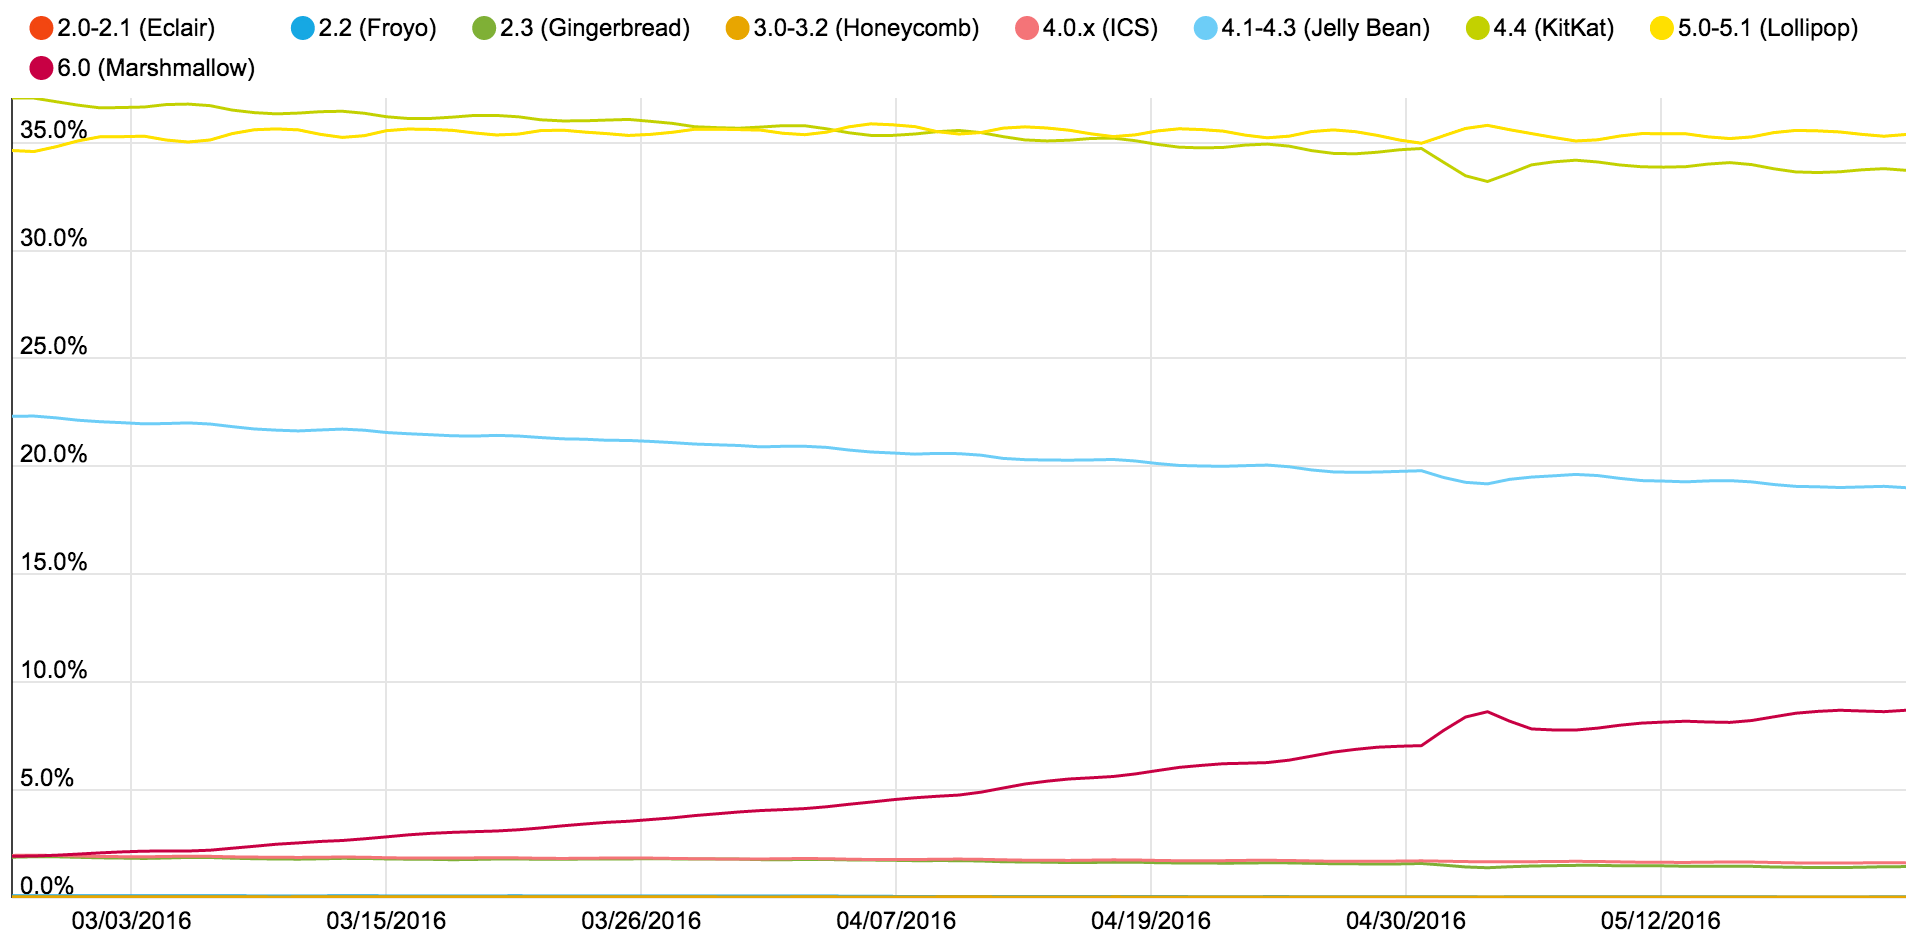
\includegraphics[width=1\textwidth]{android_version.png}
	\bicaption[fig:androidVersion]{这里将出现在插图索引中}{Android系统版本趋势}{Fig}{Android system version trendency}
\end{figure}

\begin{figure}[!htp]
	\centering
	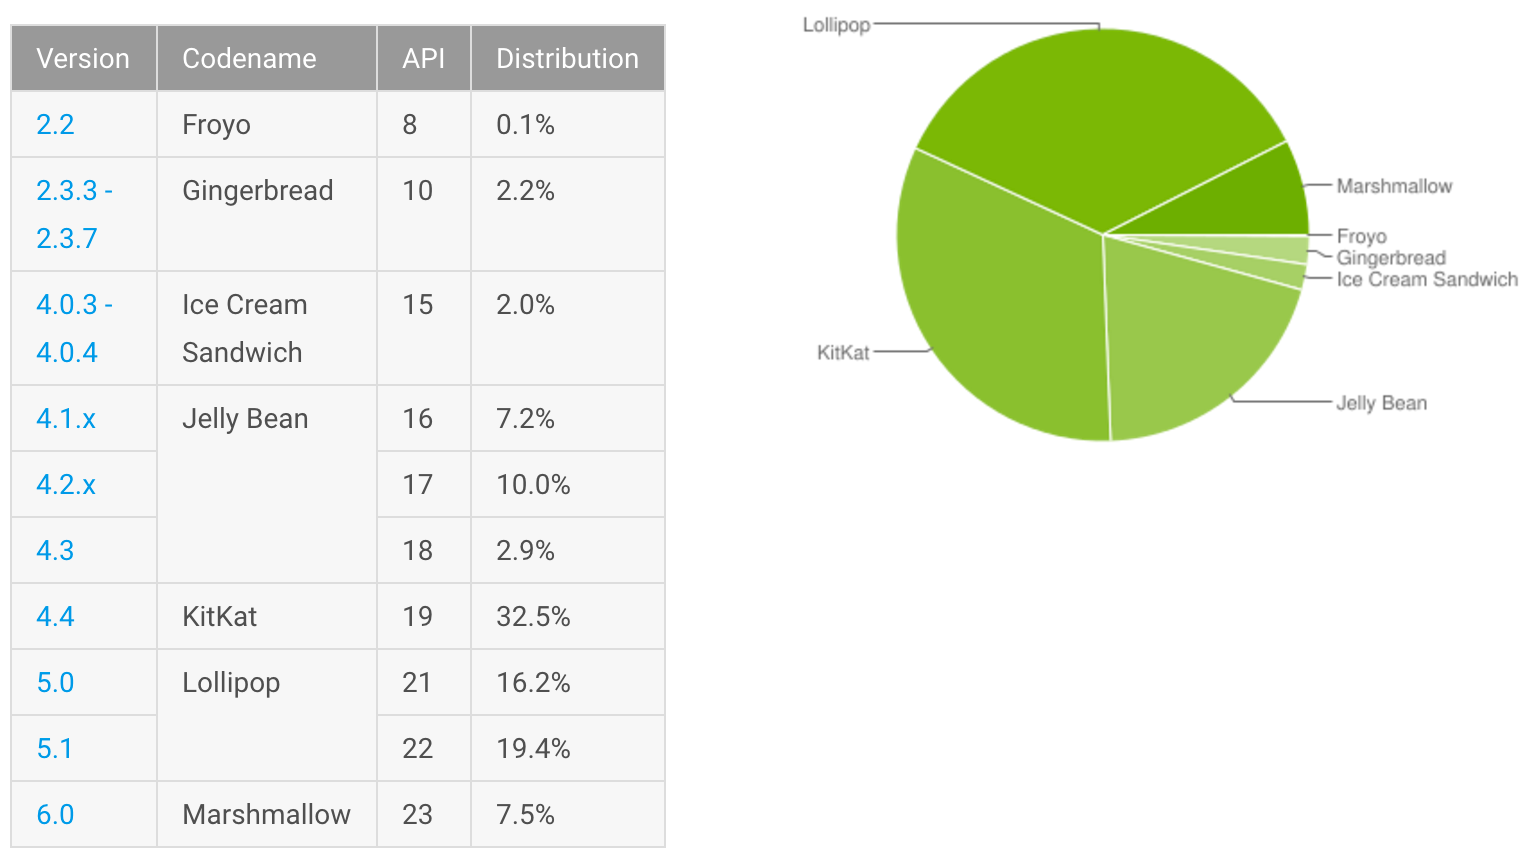
\includegraphics[width=1\textwidth]{version_distribution.png}
	\bicaption[fig:versionDistribution]{这里将出现在插图索引中}{Android系统版本分布}{Fig}{Android system version distribution}
\end{figure}

\subsection{存在的问题}
\label{subsec:exist_problem}

对于软件开发者,实现从所有用户设备中收集App的使用状况,需要考虑大规模并发、持久化存储、稳定性等各种问题,难度高而且工作量大。对于大团队或许有能力实现收集反馈信息的功能,但对于想要了解用户使用状况的独立开发者,开发这类功能的工作量过大,甚至会超过了App业务功能本身。

除此之外,开发者还要面对硬件参数各异、运行各种版本系统的用户设备,保证开发的App在碎片化的Android设备上不崩溃,并且都拥有较为良好的用户体验。开发团队在测试阶段不可能覆盖所有的Android设备,并且测试也难以覆盖所有情况。
存在一种情况,在绝大部分设备上都能正确运行的App,在某款用户量很少的Android设备上会崩溃,导致这部分用户无法正常使用。
如果能够将这款设备的App崩溃信息发送给开发者,开发者就能够定位并解决问题,通过更新App提高兼容性和稳定性。

\section{项目解决的问题}
\label{sec:solve_problem}

本文介绍的工具代号“Appetizer”,解决的是\ref{subsec:exist_problem}小节中描述的问题。“Appetizer”包括一个能够集成在Android应用中的轻量级软件开发工具包,简称为客户端SDK,和具有良好可扩展性的用于接收并处理数据的服务端程序。

Appetizer客户端SDK能够收集用户使用App的操作路径和时间,在App崩溃时收集程序调用栈和设备相关状态信息,侦测Android应用程序未响应事件,记录App每次启动时的黑白屏时间,存储这些使用信息,并在网络条件允许的情况下将收集到的信息发送到服务端。

Appetizer服务端能够持久化存储客户端SDK发送的消息,对App使用信息做处理和统计分析,展现有价值的内容给App的开发团队和运营团队,包括日活跃用户、崩溃信息分类、机型统计等处理过的数据。

Appetizer客户端SDK的特点是轻量和稳定。不使用任何第三方库,尽可能减小SDK的空间占用,减少使用该SDK的App的空间占用增加。同时保证稳定性,不会因为SDK本身的问题造成App崩溃。Appetizer服务端在架构上保证了良好的可扩展性,可以通过简单的增加服务器数量承受更大的流量压力。

\section{相关工具产品}
\label{sec:related_work}

中国市场上,提供用户行为分析统计和崩溃信息收集的商业产品主要有腾讯Bugly,友盟[4]和TalkingData[5]。他们的产品对于Android App用户行为分析方面的功能包括用户活跃度、用户构成、渠道分析、页面访问路径统计、事件转化率等,主要是对session统计得到的数据进行处理的结果,其中腾讯Bugly对应用崩溃信息分析处理功能较强。

国际市场上,提供相关功能的商业产品主要有Google FireBase,Yahoo Flurry Analytics[6]和Twitter Fabric。其中Google FireBase同时包括用户行为统计和崩溃信息收集,其他功能也较为丰富,是Google公司主推的Android开发者服务工具。Flurry Analytics可以对用户行为统计数据进行较为复杂的分析和报表输出。Fabric可以将所有用户的App崩溃信息反馈给开发团队,并且还有一整套团队测试工具进行辅助。

开源软件ACRA[9]是做Android App崩溃信息统计的工具,因为是开源软件需要使用者自己搭建服务端,崩溃信息收集功能完善并且发送的信息有很好的可定制性。

国内外的学术界也有对Android应用的用户使用行为进行分析的研究[7][8]。

\section{本章小结}

本章是整篇文章的绪论,描述了整篇文章研究的主要问题。

\ref{sec:android_ecosystem}节介绍了Android生态系统的大致流程、碎片化的问题和整个生态系统面临的问题,\ref{sec:solve_problem}节介绍了“Appetizer”的主要功能、特点和能够解决的问题,\ref{sec:related_work}节列出了国内外解决Android生态问题的相关商业产品和开源产品以及它们的特点。

%# -*- coding: utf-8-unix -*-

\chapter{背景}
\label{chap:background}

\section{Android模型}
\label{sec:androidModel}

每个操作系统都有独特的系统模型,Android系统底层基于Linux内核,同时做了许多扩展。本节介绍Android系统架构和应用模型,为阐述本文解决的问题和方法做铺垫。

\subsection{Android系统架构}

\begin{figure}[!htp]
	\centering
	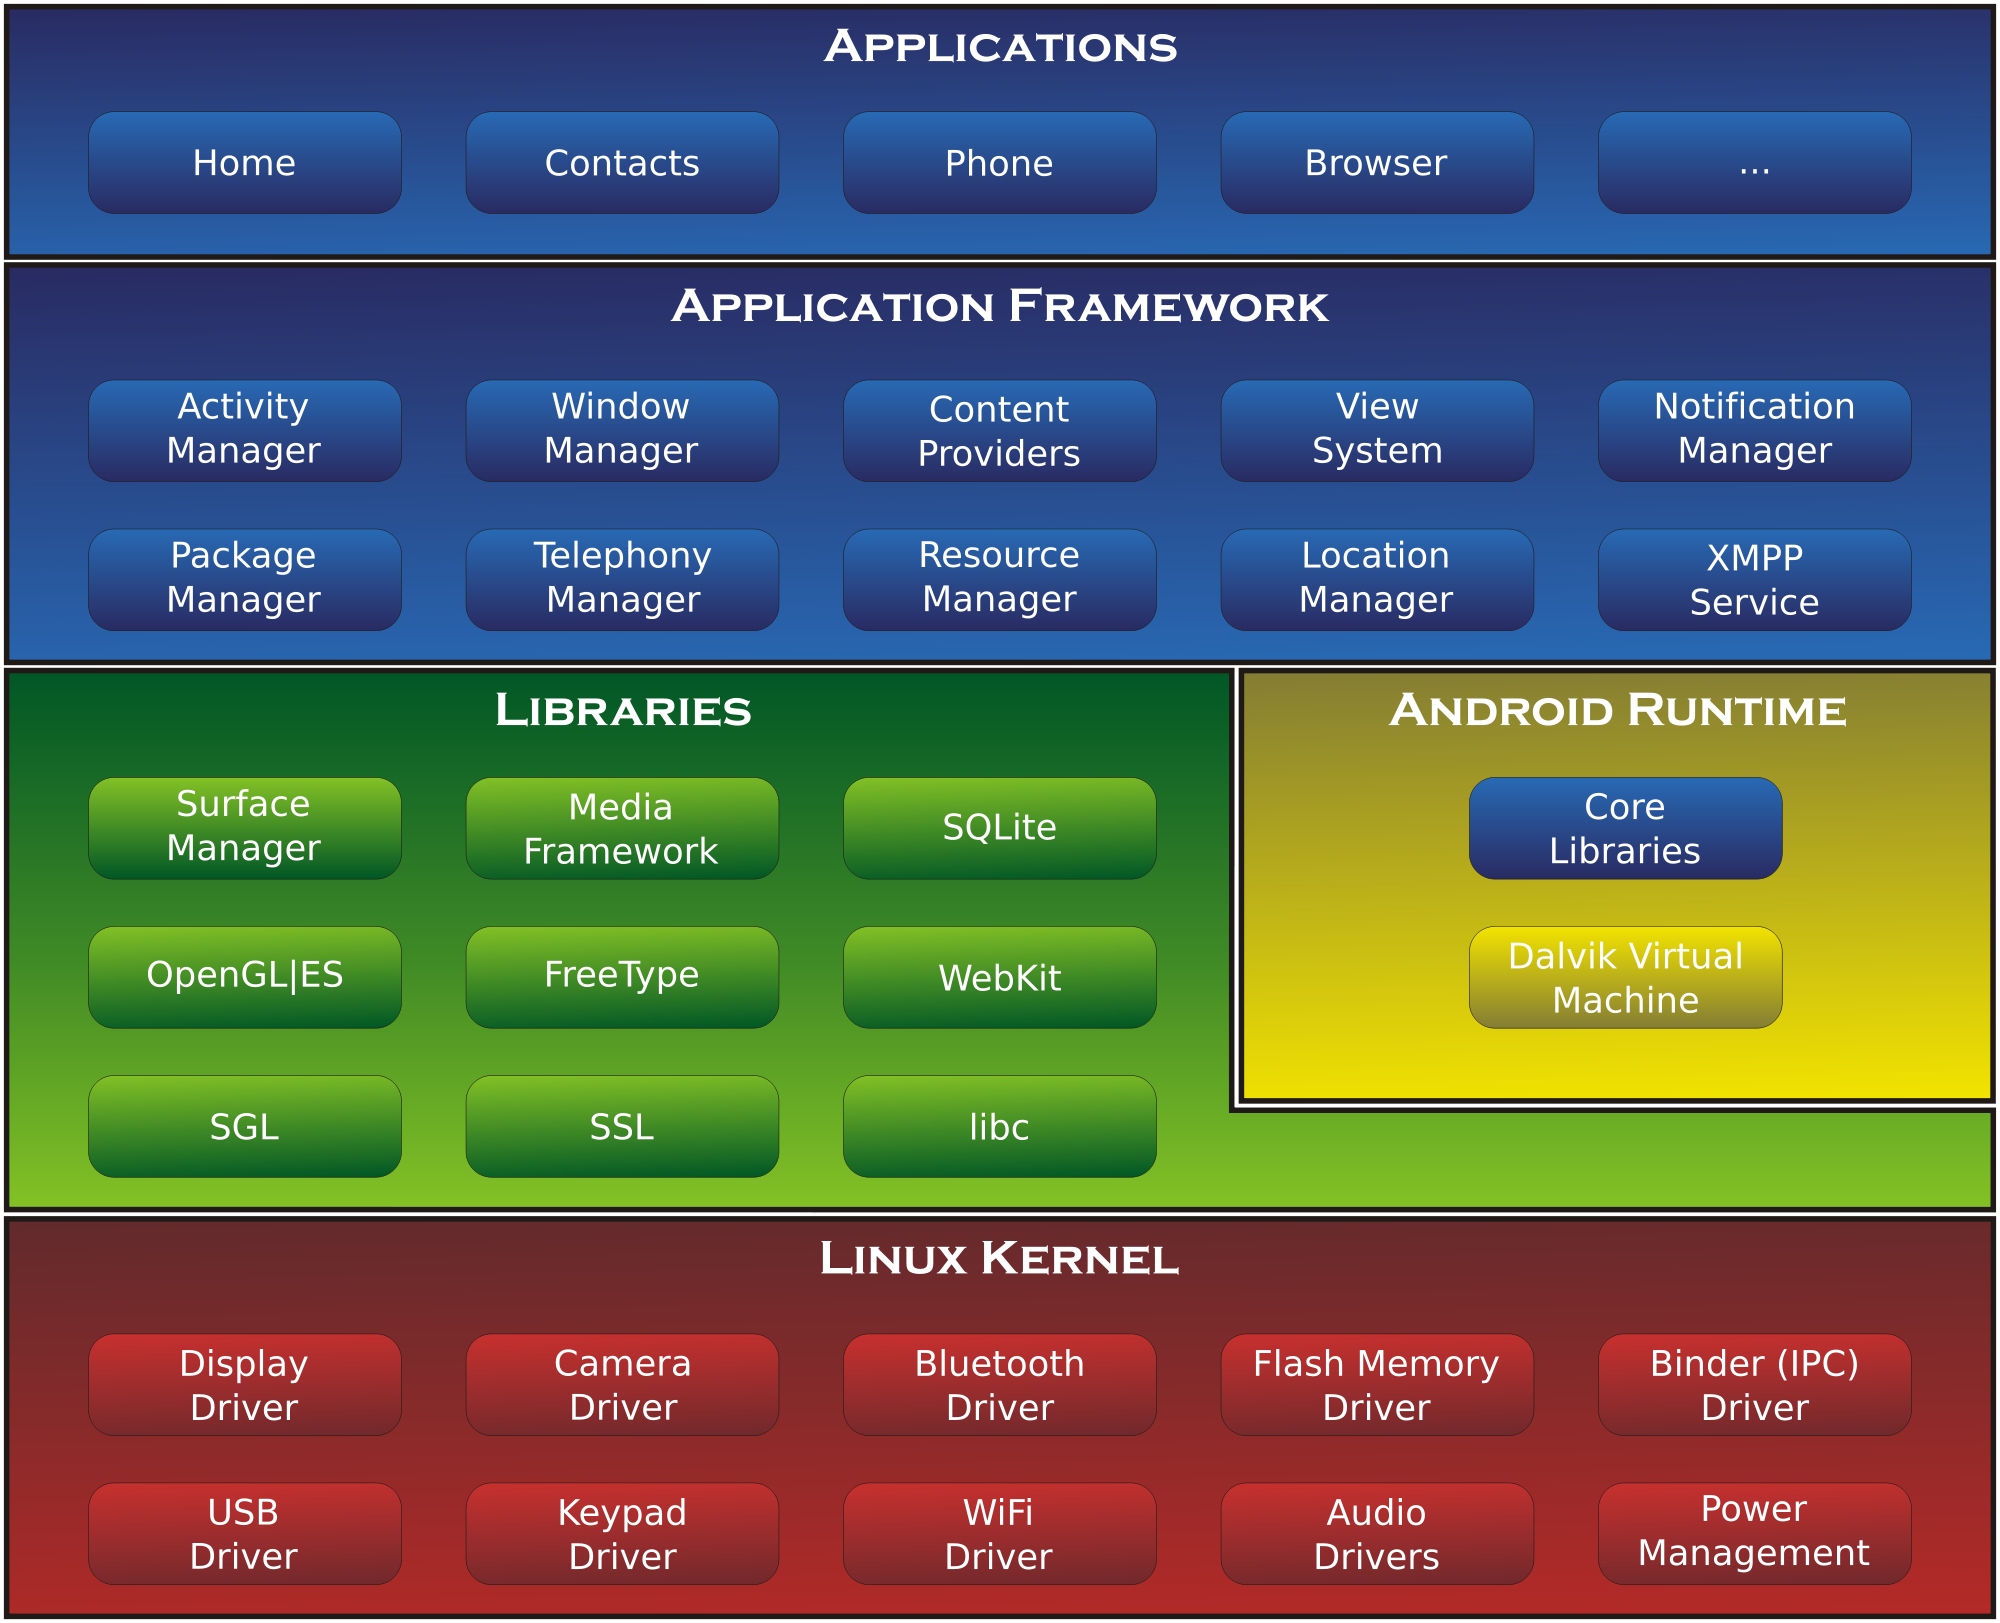
\includegraphics[width=0.9\textwidth]{AndroidSystemArchitecture.png}
	\bicaption[fig:androidSystemArchitecture]{这里将出现在插图索引中}{Android系统架构}{Fig}{Android system architecture}
\end{figure}

Android系统底层基于Linux内核,使用Linux内核文件形式的硬件驱动。Android系统中间层提供了常用的工具类库,包括轻量级数据库SQLite、浏览器引擎WebKit、图形程序接口OpenGL ES等,Android系统中间层还有Android Runtime,使用Dalvik虚拟机运行编译成字节码的程序。Android系统上层提供了窗口管理器、包管理器、资源管理器等能够让Android应用程序直接调用的工具和类库。

Android应用建立在Android系统三层架构之上,开发者通过调用Android系统提供的接口实现各种Android应用程序。图\ref{fig:androidSystemArchitecture}展现了整个Android系统的架构。

Android系统提供了名为SharedPreferences的轻量级事务性key-value存储系统,每个Android应用程序有独立的存储空间,Appetizer基于该轻量级key-value存储系统和文件系统,实现了满足原子性的轻量级二进制数据持久化消息队列。

\subsection{Android应用模型}

一台Andorid设备里的每个Android应用拥有独立的UID(User Identifier),每个App都相当于Linux中独立用户,通过复用Linux的用户级隔离机制来实现Android应用的权限控制和数据隔离。

Android应用是组件化的,每个App包括运行在前台和后台的若干组件。一个组件一般由一些Java类定义,默认多个组件在同一个Linux进程中执行,也可以通过特别的设置将前台与后台的组件运行在不同的Linux进程中。例如同一个开发团队两个App分别有一个前台Activity组件和后台Service组件,可以设置将Activity和Service拆开在两个不同的进程中运行,还可以设置两个App公用同一个Service组件,这样当两个App同时运行的时候系统中只运行了三个组件。

Android App可以注册侦听某些事件,例如网络断开、屏幕开启、电池电量不足等,当事件发生时执行一段程序。一个组件在运行时也可以产生自定义事件,并可以指定把事件告知某个或者某一类组件。

\section{反馈信息}
\label{sec:replyInfo}

Android App使用过程中会产生许多数据,其中有些数据对于开发运营团队有价值,可以帮助完善优化程序,调整运营策略,提高用户体验。

Appetizer客户端SDK会收集用户会话信息、应用崩溃信息、ANR信息和黑白屏时长信息,本节的每个小节分别介绍了各个反馈信息的具体内容,对用户体验的影响及其数据价值。

\subsection{用户会话}

Android应用程序的用户会话,可以类比网站统计中的会话,简称session,这里可以称为App session,指的是用户使用一次App的整个过程,包括起止时间,打开的内容,内容跳转的路径,每个内容浏览的时间。

在Appetizer中,“页面”定义为Android中的Activity对象跟Fragment对象,是App session中用户浏览路径的基本单元。
对于一次用户会话的具体定义如下:

\begin{itemize}
	\item 从启动应用到关闭应用
	\item 从启动应用到应用退至后台,且在后台运行时间超过30秒
	\item 从启动应用到应用停留在某个页面未跳转时间超过30秒
\end{itemize}

例如用户在一次使用App的过程中跳转了多次页面,一个用户会话会包括多个浏览路径的信息。用户在将App切换至后台运行,超过30秒后再打开,Appetizer认为这是两次不同的会话,相当于用户打开了两次App。

用户会话可以用于统计日活跃用户,周活跃用户等数据,结合设备信息可以分析出日新增用户,老用户回流等更深层次的数据,这些分析数据在网站统计中已经较为成熟。基于用户会话统计的用户活跃度分析,是应用运营、市场调研最重要的数据来源,可以帮助开发者设计追踪营销策略,了解市场,并且获得新功能的用户喜爱度反馈。

\subsection{Android应用崩溃}

Android应用程序最终以字节码的形式打包,所以通常使用能够运行在Java虚拟机上的程序语言进行开发,绝大部分Android应用使用Java语言开发,少部分使用Scala和Kotlin等JVM系语言开发,还有很少一部分使用Go语言和Swift语言开发。Android系统同时提供Native Development Kit,支持C/C++语言开发。

Android应用的崩溃可能发生在Java层,以Java抛出未被捕获的异常(Exception)或者错误(Error)的形式发生,崩溃也可能发生在Native层,本篇文章和Appetizer只考虑收集App发生在Java层的崩溃信息。

Android应用崩溃会影响用户的正常使用,崩溃的原因可能是程序逻辑代码本身的问题,设备碎片化导致的极少数设备运行问题,或者Android系统本身的问题。App崩溃会影响用户体验,在关键位置崩溃会导致App根本无法使用,崩溃会直接影响到用户量,对于用户量非常大的Android应用,低概率发生的崩溃就可能影响到成百上千万的用户。

Andorid应用崩溃信息收集功能可以及时把用户使用产生的崩溃问题告知开发团队,开发团队根据函数调用栈、设备型号、系统状态等信息对崩溃原因进行分析,及时解决问题,减少程序崩溃带来的负面影响。

\subsection{应用程序未响应}
\label{subsec:background_ANR}

Android ANR全称Application not responding(应用程序未响应),是指App运行某一段代码逻辑的时间过长,而无法响应用户的操作,通俗的说法就是程序卡死。

在Android里,应用程序的响应性是由Activity Manager和WindowManager系统服务监视的,当它监测到以下情况中的一个时,系统就会针对特定的应用程序显示ANR:

 \begin{itemize}
 	\item 在5秒内没有响应用户的输入事件
 	\item BroadcastReceiver在10秒内没有执行完毕
 \end{itemize}

Android App和用户交互的界面由主线程更新,因此主线程又称为UI线程。应用程序长时间不响应用户输入的原因,可能是UI线程在长时间执行其他任务,例如数据库操作、网络操作、复杂的计算操作,也可能是UI线程死循环或者死锁。

间歇性发生ANR会让用户感觉应用卡顿,使用体验下降,长时间发生ANR会导致用户无法与应用交互,也就无法使用App,只能让系统强制关闭该应用。收集ANR发生时的函数调用栈信息和设备实时状态,发送给开发团队,有利于开发团队解决ANR问题,提升App的用户体验。如图\ref{fig:ANRDemo}是Android应用程序发生ANR时系统的弹窗提示。

\begin{figure}[!htp]
	\centering
	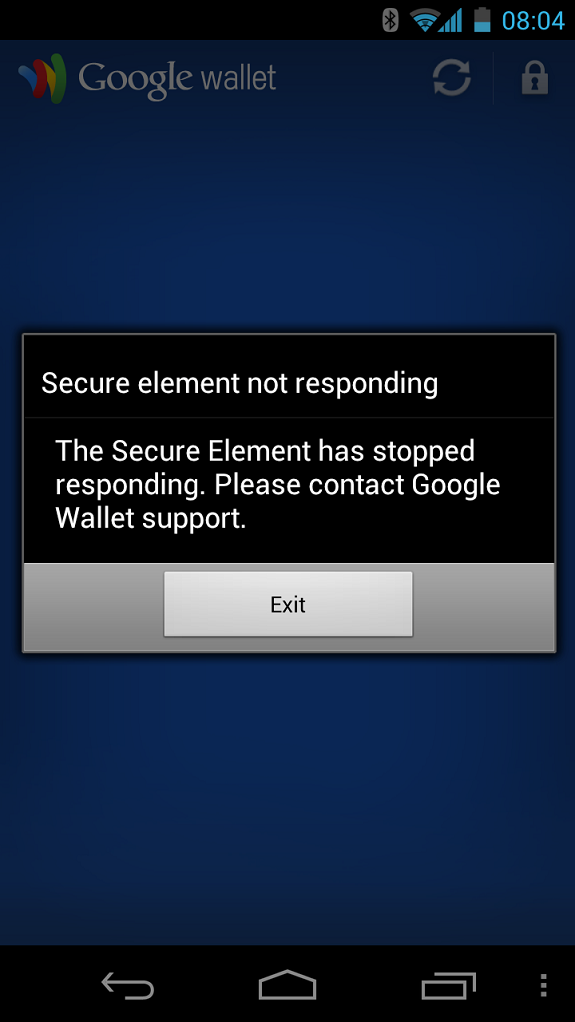
\includegraphics[width=0.3\textwidth]{ANRDemo.png}
	\bicaption[fig:ANRDemo]{这里将出现在插图索引中}{Android ANR事件}{Fig}{Android ANR event}
\end{figure}

\subsection{启动黑白屏}

Android应用在启动的时候需要加载作为入口的Activity页面。在应用启动成功之后,入口Activity的布局内容加载完成之前,显示在设备屏幕上的是Android应用的主题背景,默认的通常是黑色或者白色,在这段时间用户只能看到黑色或白色的屏幕,称为Android应用启动时的黑白屏问题。

黑白屏问题是程序启动加载需要时间导致的必然存在的问题,无法彻底解决。黑白屏持续的时间和应用程序本身、Android系统版本、硬件性能、设备实时状态都有关,一些Android应用选择透明背景或者一张图片掩盖黑白屏问题,缓解用户在这段应用启动等待时间的急躁心理,应用启动后的等待时间过长会影响用户体验。

Appetizer客户端SDK能够记录每次Android应用启动后,加载入口Activity布局文件的等待时间,也就是黑白屏时间。该数据发送给开发团队,可以让开发团队判断启动加载时间长度是否能够接受,决定是否需要对程序进行权衡和优化,以减少应用启动后的等待时间,提升App的用户体验。

\section{本章小结}

本章介绍了Appetizer项目和所解决的问题相关的技术背景,为后文的设计和实现做铺垫。

\ref{sec:androidModel}节介绍了Android系统相关的背景知识,包括Android系统架构和Android应用组件化的模型。\ref{sec:replyInfo}节介绍了Appetizer客户端SDK所收集信息的相关背景知识,以及这些信息对开发团队的价值。

%# -*- coding: utf-8-unix -*-

\chapter{客户端SDK设计与实现}
\label{chap:client}

\section{客户端SDK概要}

Appetizer客户端SDK是提供给开发者用于集成到App的部分,是完成用户使用App信息收集的必要程序。



客户端SDK的


\section{客户端SDK架构}


\section{客户端SDK实现}


\subsection{持久化消息队列}

\subsection{用户会话收集}

\subsection{崩溃信息收集}

\subsection{ANR侦测}

\subsection{黑白屏时长记录}



\section{本章小结}
%# -*- coding: utf-8-unix -*-

\chapter{服务端设计与实现}
\label{chap:server}

\section{服务端概要}
\label{sec:serverOverview}

Appetizer服务端的作用主要有三个:

\begin{itemize}
	\item 接收并存储集成了Appetizer客户端SDK的Android应用程序发送的数据。
	\item 计算分析接收的数据,得到更有价值的结果。
	\item 提供数据给开发者查看。
\end{itemize}

其中提供数据给开发者查看,是服务端提供查询API,由另外的客户端调用查询API完成展现数据给开发者的功能,该部分与核心功能关系不大,本篇文章不讨论该部分。本章主要介绍Appetizer服务端如何处理接收集成了Appetizer客户端SDK的Android应用程序发来的数据,简要介绍对数据的处理方法。

\section{服务端架构}
\label{sec:serverArch}

\begin{figure}[!htp]
	\centering
	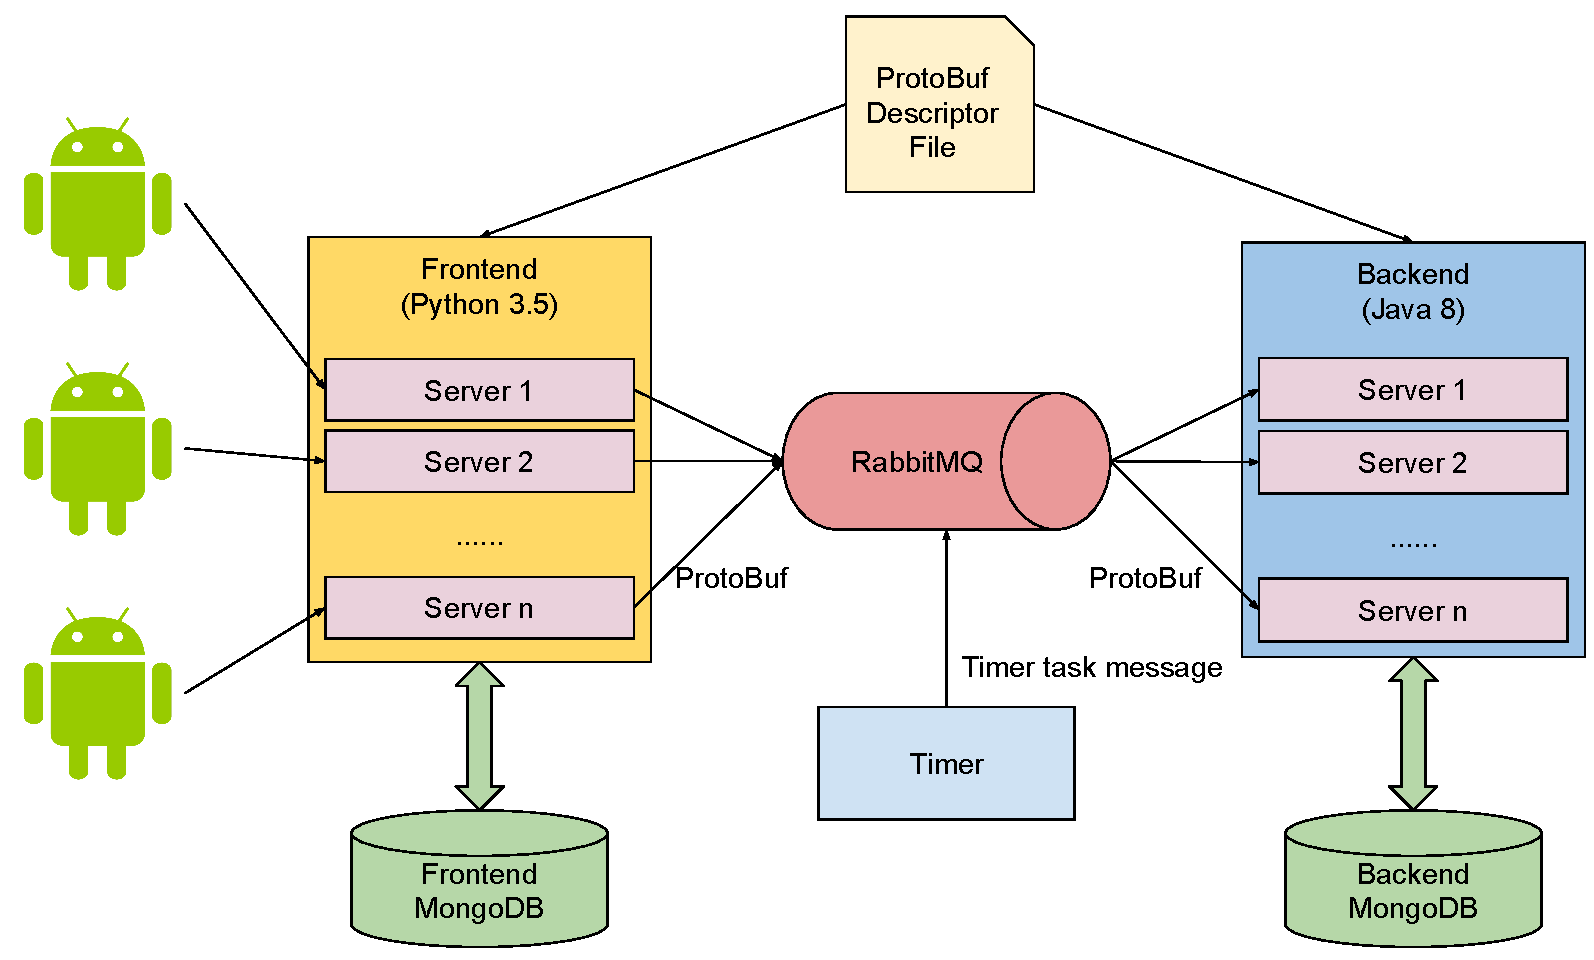
\includegraphics[width=1.0\textwidth]{AppetizerServer.pdf}
	\bicaption[fig:AppetizerServer]{这里将出现在插图索引中}{Appetizer服务端架构}{Fig}{Appetizer server architecture}
\end{figure}


如图\ref{fig:AppetizerServer}所示是服务端架构,服务端的程序主要分为前台(Frontend)和后台(Backend)两部分,其他重要的部分包括数据库(DataBase),前台后台的消息队列通信(MessageQueue)和定时器(Timer)。

前台、后台、数据库和消息队列四个部分采用的都是可扩展性良好的设计方案,并且结合每个部分处理的业务定制了专门的解决方案。

\subsection{前台}
\label{subsec:serverFrontend}

前台的主要作用是完成输入输出(IO)密集型业务。包括接收集成了Appetizer客户端SDK的Android应用程序发送的数据,对数据做简单的处理转发给后台,提供查询API供面向开发者的客户端使用,前台系统大部分时间在处理存储、网络任务,只有少量计算型任务。

Appetize服务端的前台(Frontend)部分使用Python 3.5开发,接收Andorid应用程序的数据部分基于asyncio HTTP实现。选择使用Python实现前台的首要原因Python是动态类型,提供原生Map类型便于操作JSON格式数据,可以有效提高前台业务的开发效率。Python的劣势是性能,但是前台的业务偏向输入输出(IO)密集型而不是计算密集型,因此性能的劣势不会称为整个系统运行效率的瓶颈,除此之外Python 3.5新增的协程异步关键字能很方便的开发异步程序,适合输入输出密集型的程序。

前台的业务逻辑主要包括数据格式处理、时间校准、数据库存储和数据转发到后台,业务逻辑的任务流主要使用 Python 3.5提供的async IO进行分配执行,数据库相关的操作使用第三方库motor实现,motor是一个结合async IO和MongoDB的工具库。

整个前台程序,包括HTTP请求路由、业务逻辑执行、数据库操作都支持Python的异步协程(async)机制,便于写出支持多核的不阻塞异步业务逻辑代码。

\subsection{后台}
\label{subsec:serverBackend}

后台的主要作用是持久化存储数据和完成计算密集型业务。后台接收前台做过简单处理的数据,持久化存储数据,对数据做增量型数据统计处理,定时做计算量较大的数据处理业务,处理后的数据定时发送给前台共查询API调用。

Appetizer服务端的后台(Backend)部分使用Java 8开发,主要考虑到Java不差的计算性能以及强大的工具类库,依赖的第三方库包括ProtocolBuffer、MongoDB Driver和RabbitMQ Client。
后台框架将RabbitMQ通道传来的消息分配到不同的任务执行单元,框架自动将消息内的ProtocolBuffer数据根据描述文件转成MongoDB的BSON(二进制JSON)对象,然后进行增量处理或者定时的全量处理。

定时任务的触发由另一块单独的Python程序完成,定时器同样通过RabbitMQ发送消息触发Appetizer服务端Java后台程序的定时任务,复用Java后台的消息分配机制,并且RabbitMQ生产者消费者模型有断电容错恢复机制,定时器复用消息模型增强了定时任务的稳定性。

\subsection{数据库}
\label{subsec:database}

前台和后台的数据库使用的都是MongoDB,因为Appetizer面向的数据都不是简单的用户信息,单个数据都涉及到较为复杂的多级结构,例如Android系统ROM构建信息本身还包含若干信息,直接使用JSON格式存储该信息的内容比较合适,Android系统ROM构建信息本身又是整个崩溃设备实时状态的一部分。因此存储单元为文档(Document)的NoSQL数据库MongoDB作为Appetizer服务端系统的数据库非常合适。

MongoDB的单个文档(Document)最多存4MB的数据,建议低于1MB,部分业务的数据可能大于1MB,例如统计日活跃用户的用户列表信息对于百万级用户量以上的Android应用数据会大于1MB,对于可能发生这种情况的任务,程序逻辑会对文档进行拆分。

\subsection{通信}
\label{subsec:rabbitmq}

前台和后台之间的通信采用RabbitMQ,支持多机与多机之间的生产者消费者模型消息传递。消息的内容使用ProtocolBuffer对象,前台和后台的数据模型可以使用同一份ProtocolBuffer描述文件,通过工具自动生成Python和Java的数据对象代码。为了避免写过多的后台Java模型类序列化和反序列化代码,后台部分实现了自动从ProtocolBuffer生成的Java模型类到MongoDB使用的BSON格式对象基础类型的转换。

采用生产者消费者消息模型的原因是让整个系统架构具有可伸缩性,即使某个时间段来自Android应用程序的消息数量过多,后台相比前台耗时更大,后台的任务不需要立刻反馈,无法处理的消息可以堆积在消息队列中,需要加大处理能力可以简单的增加机器,生产者消费者消息模型保证系统的稳定性和可伸缩性。

\section{服务端实现}
\label{sec:serverImplementation}

Appetizer的服务端实现偏向具体业务,不是本篇文章介绍的重点,相比于Appetizer客户端SDK的实现内容篇幅更少,主要介绍核心部分。其中时间校准对应Android客户端SDK所有带有时间信息的数据,用户统计对应Android客户端SDK收集的用户会话信息,崩溃信息处理对应Android客户端SDK收集的应用崩溃信息和应用程序未响应信息。

\subsection{时间校准}
\label{subsec:timecorrect}

时间校准是前台业务非常重要的预处理部分。集成了Appetizer客户端SDK的Android应用程序收集的数据中的时间信息,如果从远端服务器获取精确的时间存在两个问题,首先是开销太大,所有包含时间的信息都要做至少一个网络输入输出(IO)操作,其次是不能保证所有设备都在网络通畅的环境,因此Appetizer客户端SDK收集的数据从远端服务器获取时间是不可取的,只能从本地设备获取。

虽然真实情况下大部分Android系统ROM都会自动从服务器校准时间,时间比较准确,但Android设备的时间可以由用户自己修改,所以从本地获取的时间对于服务端依然是不可信的,服务端所有的时间信息需要校准到服务器的本地时间,服务器的本地时间是可控的,认为是准确可信的。

Appetizer时间校准的解决办法需要Android客户端SDK配合,对于所有涉及时间的信息,Appetizer客户端SDK在发送到服务端之前会添加发送时的本地时间数据到发送的数据包中,Appetizer服务端前台接收到数据时,服务端当前时间减去数据中发送时间得到差值,认为这个差值是服务端本地时间和Android设备本地时间的差值,再对数据中所有从Android设备获取的时间加上该差值,这样就把所有在Android设备本地获取的时间校准到服务端的时间。时间校准是Appetizer服务端前台为数不多计算量稍大的任务。

该时间校准方法依然存在两个问题:

\begin{enumerate}
	\item Android应用程序发送数据中的发送时间和服务端接收数据的服务端本地时间不是物理世界中的同一时刻,存在网络延迟的时间间隔,该间隔的大小是不确定的。
	\item Android设备可能在一次信息收集过程中记录多个时间节点之间,修改设备本地时间。例如记录用户会话信息时在开始和结束之间修改设备本地时间。
\end{enumerate} 

问题1虽然会影响时间校准的准确性,但是在本篇文章介绍的系统中是可以容忍的。因为需要精确计时的业务都是计算时间间隔,时间校准的精确程度对于时间间隔没有影响。其他需要记录时刻的业务都不需要高精度的计时,可以容忍数秒的时刻偏移。

问题2如果要彻底解决,需要Appetizer客户端SDK监听设备本地时间修改事件,还需要额外的权限。考虑到问题2发生的概率较小,即使发生也不会造成很严重的影响,因此整个系统容忍问题2的存在。

\subsection{用户统计}
\label{subsec:usercomputing}

用户统计是能够依靠简单的数字直观展现Android应用程序用户活跃趋势的度量维度。从宏观上考虑,用户活跃度主要受应用体验和运营策略两个因素的影响,应用体验包括界面设计、应用卡顿、应用崩溃等因素,Appetizer客户端SDK可以收集这些数据,开发和运营团队可以根据用户统计对应用界面和运营方式进行调整。

用户统计的业务实现主要包括两部分,实时用户使用量和以天为单位的日活跃用户(DAU)、日活跃新增用户(DNU)、日活跃老用户(DOU)。

实时使用量的统计难以做到精确,因为实时统计需要每台设备在使用的过程中能够顺利发送数据到Appetizer服务端,网络环境不允许的设备数据的实时性遭到了破坏,因此Appetizer服务端实现的实时使用量统计会比真正的实时使用量低。
实时使用量的业务在后台实现,前台转发时间校准后的用户会话数据到后台,实时使用量不需要考虑同一个用户多次开启应用程序合并次数,后台在存储用户会话数据的同时进行增量统计,定时器间隔五分钟触发定时任务,后台将每个Android应用程序近7天的以小时为单位的应用使用量发送到前台,前台更新接收的数据到前台数据库,供查询API调用。

日活跃相关数据业务统计更为复杂,会话数据需要和设备信息进行关联。定时器每天触发日活跃相关数据任务一次,对于每个应用程序,后台程序对当日时间内的会话数据以设备ID为键进行聚合统计,得到该应用程序日活跃用户列表。Appetizer对于“老用户”的定义为7天之内使用过应用程序的用户,因此日活跃新增用户(DNU)通过日活跃用户(DAU)列表减去之前7天的日活跃用户(DAU\_last\_7\_days)列表计算得到。日活跃新增(DNU)用户通过日活跃用户(DAU)列表减去日活跃老用户(DOU)列表计算得到。三个日活跃相关数据计算得到后只发送用户数量给前台,因为前台只关注用户数量不需要具体的用户列表。

\ref{subsec:database}小节介绍了MongoDB单个文档(Document)支持的最大空间为4MB,用户统计的用户列表作为一个List对象存储在一个文档(Document)中,List中的元素是设备ID,因此当某个Android应用的日活跃用户超过一百万时,存储一百万个设备ID在一个List会造成整个文档的大小超过4MB。用户统计业务逻辑考虑到这个问题,对于用户量较多的单个Android应用程序进行日活跃度相关的计算时,单个文档过大会进行分文档存储。

\subsection{崩溃信息处理}
\label{subsec:crashcomputing}

不同的Android设备发送的崩溃信息可能是由于同一个原因导致的,因此对崩溃信息做聚类可以更直观的展现给开发者查看,每个崩溃原因作为一个独立的事项,还包括该崩溃发生的设备系统分布、机型分布等有价值的信息,可以用来判断是否是设备或者系统的原因而不是程序本身造成的应用崩溃。

Android应用崩溃根据函数调用栈的信息进行分类,从调用栈最底层开始到最顶层看做一个单项链表,链表节点内容为文件名、函数名、行号的元组。链表节点主要分为两类,一类是开发者写的Android应用程序部分的代码,特征为包名开头为项目的名字,可以直接通过包名进行区分,另一类是Android系统本身的代码、Android支持库(support library)的代码和其他第三方库的代码,特征为包名开头是android、java或者项目目录Manifest里依赖的第三方库的包名。

两个崩溃信息根据满足以下规则2或规则3中的一个并且满足规则1,则认为是同一个崩溃原因,否则认为是不同的崩溃原因:

\begin{enumerate}
	\item 首先抛出的异常或者错误的类名相同。
	\item 链表的第一个节点如果是开发者的代码,则从第一个节点依次到首个Android系统或者支持库的代码节点之前,节点内容全部相同。
	\item 链表的第一个节点如果是Android系统或者支持库的代码,则从第一个节点依次到首个开发者的代码节点(包括首个开发者的代码节点),节点内容全部相同。
\end{enumerate}

相同的崩溃原因造成的崩溃集合,称为一个崩溃项。Appetizer服务端接收到Android设备发送的崩溃信息后,会做如下处理:

\begin{enumerate}
	\item 找到该崩溃信息对应的Android应用程序。
	\item 将崩溃信息的哈希值和该Android应用程序中已有崩溃信息的哈希值进行对比,如果存在相同的哈希值,将此次崩溃加入到该崩溃项的列表中,业务逻辑程序结束。
	\item 根据上述的链表匹配规则和该Android应用程序中的每个崩溃信息链表进行对比,如果判断为同一个崩溃原因,将此次崩溃加入到该崩溃项的列表中,业务逻辑程序结束。
	\item 创建新的崩溃项,将此次崩溃加入到新的崩溃项的列表中。
\end{enumerate} 

步骤2的哈希值相当于崩溃信息索引,通常情况下一个Android应用的大部分崩溃信息都是由少部分崩溃原因造成的,如果对于每个崩溃信息都进行链表匹配算法会造成巨大的开销,因此通过哈希索引崩溃信息可以大幅提高业务流程处理的的速度。

在崩溃信息加入到崩溃项中之后,会对该崩溃项的设备分布、版本分布统计信息做增量计算,可以给开发者提供每个崩溃项的设备分布统计和版本分布统计数据。

\section{本章小结}

本章内容主要介绍了Appetizer服务端的架构以及核心业务功能,服务端是整个系统不可或缺的一部分,用于存储、处理Appetizer客户端收集的数据,提炼出有价值的信息提供给开发者和运营团队进行查看。

\ref{sec:serverOverview}节介绍了服务端收集Android设备发送的数据、对数据进行处理、提供给开发者和运营团队查看处理后数据的三个主要功能。

\ref{sec:serverArch}节介绍了服务端整体架构,对各个组件的技术选型原因进行了分析。
\ref{subsec:serverFrontend}小节介绍了前台系统的主要功能,解释了前台业务偏向输入输出(IO)密集型的特点,分析了选择Python实现前台系统的原因以及前台在实现上选择工具库做出的权衡。
\ref{subsec:serverBackend}小节介绍了后台系统的主要功能,后台业务偏向计算密集型的特点,说明了后台系统选择Java开发的原因,消息队列RabbitMQ在后台系统的作用和定时器的设计。
\ref{subsec:database}小节介绍了MongoDB的优势以及Appetizer服务端选择MongoDB作为前台和后台数据库的原因,还说明了可能需要拆分文档的应用场景。
\ref{subsec:rabbitmq}小节介绍了Appetizer服务端前台和后台之间的通信机制,通信传递的内容采用ProtocolBuffer同时具备性能和便于开发的优势,以及相关通信架构提供的系统可伸缩性和可扩展性。

\ref{sec:serverImplementation}节介绍了Appetizer服务端有展现价值的部分。
\ref{subsec:timecorrect}小节介绍了在Appetizer整个业务流程中发生的时间偏差的原因,Appetizer客户端SDK只从本地设备获取不可信时间,设计并实现了依靠客户端SDK和服务端合作的时间校准方法,分析了该方法可能发生的问题,得到该时间校准方法有效可行的结论。
\ref{subsec:usercomputing}小节介绍了Appetizer核心功能用户统计的价值、作用和实现方法。
\ref{subsec:crashcomputing}小节介绍了Appetizer另一个核心功能崩溃信息处理的设计实现,描述了一种对Android应用崩溃信息的原因进行分类的方法。

%# -*- coding: utf-8-unix -*-

\chapter{评估测试}
\label{chap:evaluation}

评估测试部分主要涉及Appetizer客户端SDK在Android设备上的影响,因为对于使用Appetizer客户端SDK的开发者来说,他们关心的主要问题是SDK对于原来Android应用程序的性能影响、空间占用应用等,Appetizer服务端是隐藏的黑盒。
因此本篇文章介绍的Appetizer整套系统中,和同类产品相比核心竞争力之一是Appetizer客户端SDK的各项指标。

\section{功能对比}

功能列表


\section{SDK空间占用对比}

对于做用户数据收集的Android SDK,集成到Android应用程序占用的额外空间同样是一个重要指标。因为作为第三方工具库,本身占用空间的增大会造成所有集成该工具库的占用空间变大,影响范围较广,因此第三方工具库的占用空间越小越好。

表\ref{tab:SDK_size}展示的是Appetizer和同类Android SDK占用空间的数据,表中列举的产品中ACRA的功能覆盖面最小,本文介绍的Appetizer客户端SDK在功能覆盖上是ACRA的超集,减少部分崩溃信息可定制化的功能,增加了注入用户会话信息、Andorid程序未响应侦测等功能,但是占用空间更小。其他产品在功能上和Appetizer相比各有千秋,占用空间都远超Appetizer客户端SDK。

图\ref{fig:SDK_size}展现的是Appetizer和同类Android SDK占用空间倒数的柱状图,可以等价于各个产品在占用空间上的得分,更直观的展现了Appetizer客户端SDK轻量级的优势。

\begin{table}[!hpb]
	\centering
	\bicaption[tab:SDK_size]{指向一个表格的表目录索引}{产品SDK占用空间表}{Table}{Product SDK size table}
	\begin{tabular}{@{}llr@{}} \toprule
		Product & Version &Size \\ \midrule
		Appetizer &v0.1& 71 kB \\
		Umeng&v6.0.1& 301 kB \\
		TalkingData&v2.2.25& 386 kB \\
		ACRA&v4.9.0& 152 kB \\
		Flurry Analytics&v6.3.1& 260 kB \\ \bottomrule
	\end{tabular}
\end{table}

\begin{figure}[!htp]
	\centering
	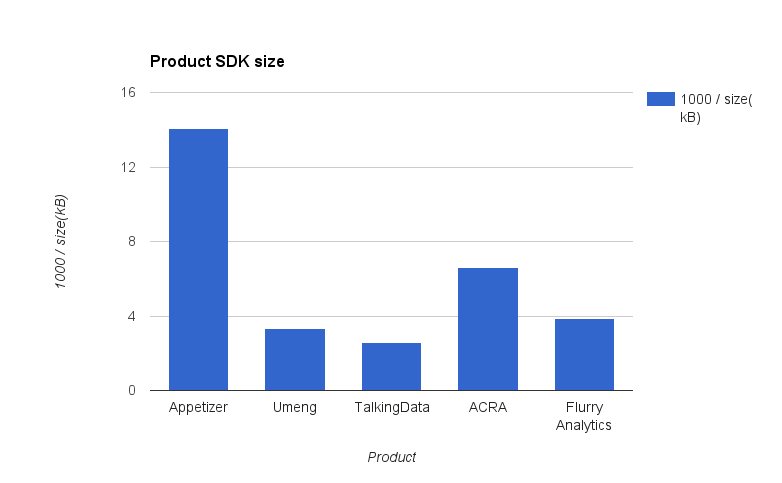
\includegraphics[width=0.9\textwidth]{SDK_size.png}
	\bicaption[fig:SDK_size]{这里将出现在插图索引中}{产品SDK占用空间}{Fig}{Product SDK size}
\end{figure}

\section{性能对比}





\section{本章小节}


%# -*- coding: utf-8-unix -*-

\begin{summary}

本篇文章介绍了Appetizer,是一个能够收集Android平台用户使用应用程序的行为、应用程序卡顿、应用程序溃信息的系统。Appetizer包括一个能够集成在Android应用中的轻量级软件开发工具包,和一套具有良好可扩展性的用于接收并处理数据的服务端程序。

第\ref{chap:intro}章绪论介绍了Android生态系统的构成,Android生态系统中存在的系统碎片化和设备碎片化的问题,以及碎片化所带来的影响,分析了Android生态系统中开发者和用户之间存在使用体验反馈难的问题,解释用户使用信息对于Android应用程序开发和运营的价值。根据Android生态系统中存在的问题,提出了Appetizer的作用就是解决这些问题,同时罗列了相关同类产品。

第\ref{chap:background}章背景介绍了Android系统和应用的架构模型及平台特点,是理解Appetizer客户端SDK设计方案的背景知识。还介绍了Appetizer客户端SDK反馈信息的内容、原因和作用。

第\ref{chap:client}章是整篇文章的核心章节,该章描述了客户端SDK的架构、设计方案以及制定出最后设计的权衡过程,架构体现了Appetizer客户端SDK相比于同类产品更加轻量化的特点。该章着重介绍了Appetizer客户端SDK关键功能的实现方式,包括网络模块的选择,持久化队列的设计实现以及如何同时保证原子性、一致性和轻量化的,用户会话收集和崩溃信息收集的实现方式,应用程序未响应(ANR)的巧妙实现方式和黑白屏时长记录。

第\ref{chap:server}章介绍了接收Appetizer客户端SDK所收集信息的服务端,着重介绍了服务端的架构设计和方案选择过程中的权衡,分别对前台(Frontend)、后台(Backend)、数据库和前后台通信的技术方案选择设计与实现进行了详细介绍。业务部分,在时间校准上设计了一种适合Appetizer应用场景的解决方案,还介绍了用户统计的实现方法,以及对崩溃信息进行快速归类的算法。

第\ref{chap:evaluation}章对Appetizer客户端SDK进行了测试,从功能上和SDK所占用的空间大小上和同类产品进行对比,结论是Appetizer客户端SDK收集的Android应用程序使用信息覆盖面较广,而且SDK占用空间明显小于同类产品,具有轻量化的优势。还从性能角度对Appetizer客户端SDK的初始化、用户会话收集、应用程序未响应(ANR)侦测功能进行了测试实验,在多个系统版本的主流Android设备上的实验结果表明,集成Appetizer客户端SDK对Android应用程序性能影响小到可以忽略,不会影响用户体验。

整篇文章从需求背景、技术背景、设计实现、功能对比和性能测试等多个角度介绍了Appetizer,展现了集成Appetizer客户端SDK能够以较小的代价解决Android开发者的痛点,开发者可以从Appetizer服务端获取到提炼过的有价值的数据,并且Appetizer和同类产品相比在轻量化和信息收集覆盖面等方面具有一定优势。

在技术角度上,本文提出并介绍了基于Android SharedPreferences和文件系统,保证原子性和一致性的轻量级持久化队列,以及客户端SDK收集信息在服务端的时间校准方法,具有一定创新性和实用价值,可以供其他开发者进行参考。

\end{summary}


% \appendix	% 使用英文字母对附录编号,重新定义附录中的公式、图图表编号样式
% \renewcommand\theequation{\Alph{chapter}--\arabic{equation}}	
% \renewcommand\thefigure{\Alph{chapter}--\arabic{figure}}
% \renewcommand\thetable{\Alph{chapter}--\arabic{table}}
% \renewcommand\thealgorithm{\Alph{chapter}--\arabic{algorithm}}

%% 附录内容,本科学位论文可以用翻译的文献替代。
% %# -*- coding: utf-8-unix -*-
\chapter{搭建模板编译环境}

\section{安装TeX发行版}

\subsection{Mac OS X}

Mac用户可以从MacTeX主页\footnote{\url{https://tug.org/mactex/}}下载MacTeX 2015。
也可以通过brew包管理器\footnote{\url{http://caskroom.io}}安装MacTeX 2015。

\begin{lstlisting}[basicstyle=\small\ttfamily, numbers=none]
brew cask install mactex
\end{lstlisting}

\subsection{Linux}

建议Linux用户使用TeXLive主页\footnote{\url{https://www.tug.org/texlive/}}的脚本来安装TeXLive 2015。
以下命令将把TeXLive发行版安装到当前用户的家目录下。
若计划安装一个供系统上所有用户使用的TeXLive,请使用root账户操作。

\begin{lstlisting}[basicstyle=\small\ttfamily, numbers=none]
wget http://mirror.ctan.org/systems/texlive/tlnet/install-tl-unx.tar.gz
tar xzvpf install-tl-unx.tar.gz
cd install-tl-20150411/
./install-tl
\end{lstlisting}

\section{安装中文字体}

\subsection{Mac OS X、Deepin}

Mac和Deepin用户双击字体文件即可安装字体。

\subsection{RedHat/CentOS用户}

RedHat/CentOS用户请先将字体文件复制到字体目录下,调用fc-cache刷新缓存后即可在TeXLive中使用新字体。

\begin{lstlisting}[basicstyle=\small\ttfamily, numbers=none]
mkdir ~/.fonts
cp *.ttf ~/.fonts				# 当前用户可用新字体
cp *.ttf /usr/share/fonts/local/	# 所有用户可以使用新字体
fc-cache -f
\end{lstlisting}


% %# -*- coding: utf-8-unix -*-
%% app2.tex for SJTU Master Thesis
%% based on CASthesis
%% modified by wei.jianwen@gmail.com
%% version: 0.3a
%% Encoding: UTF-8
%% last update: Dec 5th, 2010
%%==================================================

\chapter{Maxwell Equations}

选择二维情况,有如下的偏振矢量:
\begin{subequations}
  \begin{eqnarray}
    {\bf E}&=&E_z(r,\theta)\hat{\bf z} \\
    {\bf H}&=&H_r(r,\theta))\hat{ \bf r}+H_\theta(r,\theta)\hat{\bm
      \theta}
  \end{eqnarray}
\end{subequations}
对上式求旋度:
\begin{subequations}
  \begin{eqnarray}
    \nabla\times{\bf E}&=&\frac{1}{r}\frac{\partial E_z}{\partial\theta}{\hat{\bf r}}-\frac{\partial E_z}{\partial r}{\hat{\bm\theta}}\\
    \nabla\times{\bf H}&=&\left[\frac{1}{r}\frac{\partial}{\partial
        r}(rH_\theta)-\frac{1}{r}\frac{\partial
        H_r}{\partial\theta}\right]{\hat{\bf z}}
  \end{eqnarray}
\end{subequations}
因为在柱坐标系下,$\overline{\overline\mu}$是对角的,所以Maxwell方程组中电场$\bf E$的旋度:
\begin{subequations}
  \begin{eqnarray}
    &&\nabla\times{\bf E}=\mathbf{i}\omega{\bf B} \\
    &&\frac{1}{r}\frac{\partial E_z}{\partial\theta}{\hat{\bf
        r}}-\frac{\partial E_z}{\partial
      r}{\hat{\bm\theta}}=\mathbf{i}\omega\mu_rH_r{\hat{\bf r}}+\mathbf{i}\omega\mu_\theta
    H_\theta{\hat{\bm\theta}}
  \end{eqnarray}
\end{subequations}
所以$\bf H$的各个分量可以写为:
\begin{subequations}
  \begin{eqnarray}
    H_r=\frac{1}{\mathbf{i}\omega\mu_r}\frac{1}{r}\frac{\partial
      E_z}{\partial\theta } \\
    H_\theta=-\frac{1}{\mathbf{i}\omega\mu_\theta}\frac{\partial E_z}{\partial r}
  \end{eqnarray}
\end{subequations}
同样地,在柱坐标系下,$\overline{\overline\epsilon}$是对角的,所以Maxwell方程组中磁场$\bf H$的旋度:
\begin{subequations}
  \begin{eqnarray}
    &&\nabla\times{\bf H}=-\mathbf{i}\omega{\bf D}\\
    &&\left[\frac{1}{r}\frac{\partial}{\partial
        r}(rH_\theta)-\frac{1}{r}\frac{\partial
        H_r}{\partial\theta}\right]{\hat{\bf
        z}}=-\mathbf{i}\omega{\overline{\overline\epsilon}}{\bf
      E}=-\mathbf{i}\omega\epsilon_zE_z{\hat{\bf z}} \\
    &&\frac{1}{r}\frac{\partial}{\partial
      r}(rH_\theta)-\frac{1}{r}\frac{\partial
      H_r}{\partial\theta}=-\mathbf{i}\omega\epsilon_zE_z
  \end{eqnarray}
\end{subequations}
由此我们可以得到关于$E_z$的波函数方程:
\begin{eqnarray}
  \frac{1}{\mu_\theta\epsilon_z}\frac{1}{r}\frac{\partial}{\partial r}
  \left(r\frac{\partial E_z}{\partial r}\right)+
  \frac{1}{\mu_r\epsilon_z}\frac{1}{r^2}\frac{\partial^2E_z}{\partial\theta^2}
  +\omega^2 E_z=0
\end{eqnarray}

% %# -*- coding: utf-8-unix -*-
\chapter{从 \CJKLaTeX 转向 \XeTeX }
\label{chap:whydvipdfm}

我习惯把v0.2a使用dvipdfmx编译的硕士学位论文模板称为“ \CJKLaTeX 模板”,而这个使用 \XeTeX 引擎(xelatex程序)处理的模板则被称为“{\XeTeX/\LaTeX}模板”。
从 \CJKLaTeX 模板迁移到{\XeTeX\LaTeX}模板的好处有下:
\begin{enumerate}
\item[\large\smiley] 搭建 \XeTeX 环境比搭建 \CJKLaTeX 环境更容易;
\item[\large\smiley] 更简单的字体控制;
\item[\large\smiley] 完美支持PDF/EPS/PNG/JPG图片,不需要“bound box(.bb)”文件;
\item[\large\smiley] 支持OpenType字体的复杂字型变化功能;
\end{enumerate}

当然,这也是有代价的。由于 \XeTeX 比较新,在我看来,使用 \XeTeX 模板所必须付出的代价是:

\begin{enumerate}
\item[\large\frownie] 必须把你“古老的” \TeX 系统更新为较新的版本。TeXLive 2012和CTeX 2.9.2能够编译这份模板,而更早的版本则无能为力。
\item[\large\frownie] 需要花一些时间把你在老模板上的工作迁移到新模板上。
\end{enumerate}

第一条就看你如何取舍了,新系统通常意味着更好的兼容性,值得升级。而转换模板也不是什么特别困难的事情,可以这样完成:

\begin{enumerate}
\item 备份你要转换的源文件,以防你的工作成果丢失;
\item 将你原来的tex以及bib文件另存为UTF-8编码的文件。iconv、vim、emacs、UEdit等等工具都可以完成。WinEdt对文件编码识别功能很差(到了v6.0还是如此),不推荐作为字符编码转换工具;
\item 将diss.tex导言区中的内容替换为XeTeX模板diss.tex导言区的内容;
\item 将你对原先导言区的修改,小心翼翼地合并到新的导言区中;
\item 使用XeTeX模板中的GBT7714-2005NLang.bst替换原有的bst文件,新的bst文件只是将字符编码转换为UTF-8;
\item 删除bouding box文件;
\item 使用本文\ref{sec:process}介绍的方法,重新编译文档;
\end{enumerate}


% %# -*- coding: utf-8-unix -*-
\chapter{模板更新记录}
\label{chap:updatelog}

\textbf{2015年6月19日} v0.9发布,适配ctex 2.x宏包,需要使用TeXLive 2015编译。

\textbf{2015年3月15日} v0.8发布,使用biber/biblatex组合替代 \BibTeX ,带来更强大稳定的参考文献处理能力;添加enumitem宏包增强列表环境控制能力;完善宏包文字描述。

\textbf{2015年2月15日} v0.7发布,增加盲审选项,调用外部工具插入扫描件。

\textbf{2015年2月14日} v0.6.5发布,修正一些小问题,缩减git仓库体积,仓库由sjtu-thesis-template-latex更名为SJTUThesis。

\textbf{2014年12月17日} v0.6发布,学士、硕士、博士学位论文模板合并在了一起。

\textbf{2013年5月26日} v0.5.3发布,更正subsubsection格式错误,这个错误导致如"1.1 小结"这样的标题没有被正确加粗。

\textbf{2012年12月27日} v0.5.2发布,更正拼写错误。在diss.tex加入ack.tex。

\textbf{2012年12月21日} v0.5.1发布,在 \LaTeX 命令和中文字符之间留了空格,在Makefile中增加release功能。

\textbf{2012年12月5日} v0.5发布,修改说明文件的措辞,更正Makefile文件,使用metalog宏包替换xltxtra宏包,使用mathtools宏包替换amsmath宏包,移除了所有CJKtilde(\verb+~+)符号。

\textbf{2012年5月30日} v0.4发布,包含交大学士、硕士、博士学位论文模板。模板在\href{https://github.com/weijianwen/sjtu-thesis-template-latex}{github}上管理和更新。

\textbf{2010年12月5日} v0.3a发布,移植到 \XeTeX/\LaTeX 上。

\textbf{2009年12月25日} v0.2a发布,模板由CASthesis改名为sjtumaster。在diss.tex中可以方便地改变正文字号、切换但双面打印。增加了不编号的一章“全文总结”。
添加了可伸缩符号(等号、箭头)的例子,增加了长标题换行的例子。

\textbf{2009年11月20日} v0.1c发布,增加了Linux下使用ctex宏包的注意事项、.bib条目的规范要求,
修正了ctexbook与listings共同使用时的断页错误。

\textbf{2009年11月13日} v0.1b发布,完善了模板使用说明,增加了定理环境、并列子图、三线表格的例子。

\textbf{2009年11月12日} 上海交通大学硕士学位论文 \LaTeX 模板发布,版本0.1a。



\backmatter	% 文后无编号部分 

%% 参考资料
\printbibliography[heading=bibintoc]

%% 致谢、发表论文、申请专利、参与项目、简历
%% 用于盲审的论文需隐去致谢、发表论文、申请专利、参与的项目
\makeatletter

%%
% "研究生学位论文送盲审印刷格式的统一要求"
% http://www.gs.sjtu.edu.cn/inform/3/2015/20151120_123928_738.htm

% 盲审删去删去致谢页
\ifsjtu@review\relax\else
  %# -*- coding: utf-8-unix -*-
\begin{thanks}

这篇论文的完成,为我的本科学习生活画上了句号。

首先要感谢我的母亲,对我从小到大的抚养和教育,以及在我本科前半段时间对我的经济支持。

感谢戚正伟老师给我在实验室进行学习深造的机会,以及在学术上对我的指导和帮助。

感谢夏鸣远博士在毕业设计上对我的指导和帮助,让我开阔了视野。感谢龚路学长在项目开发、系统设计和编码规范上对我的指导和帮助。

感谢室友和Trusted Cloud实验室的同学,在技术上的探讨和生活上的帮助。

感谢上海交通大学软件学院的王赓老师、肖凯老师、李垚学长、李强学长在我本科期间对我的项目指导,让我能在本科低年级的时候接触到复杂的项目开发。

感谢以上所有人,因为有你们我才能顺利完成本科学业。

\end{thanks}
 	  %% 致谢
\fi

% 盲审论文中,发表学术论文及参与科研情况等仅以第几作者注明即可,不要出现作者或他人姓名
%\ifsjtu@review\relax
%  %# -*- coding: utf-8-unix -*-

\begin{publications}{99}
    \item\textsc{第一作者}. {中文核心期刊论文}, 2007.  
    \item\textsc{第一作者}. {EI国际会议论文}, 2006.
\end{publications}

%  %# -*- coding: utf-8-unix -*-

\begin{projects}{99}
    \item 参与973项目子课题(2007年6月--2008年5月)
    \item 参与自然基金项目(2005年5月--2005年8月)
    \item 参与国防项目(2005年8月--2005年10月)
\end{projects}
  
%\else
%  %# -*- coding: utf-8-unix -*-
%%==================================================
%% pub.tex for SJTUThesis
%% Encoding: UTF-8
%%==================================================

\begin{publications}{99}
    \item\textsc{Chen H, Chan C~T}. {Acoustic cloaking in three dimensions using acoustic metamaterials}[J]. Applied Physics Letters, 2007, 91:183518.
    \item\textsc{Chen H, Wu B~I, Zhang B}, et al. {Electromagnetic Wave Interactions with a Metamaterial Cloak}[J]. Physical Review Letters, 2007, 99(6):63903.
\end{publications}
	      %% 发表论文
%  %# -*- coding: utf-8-unix -*-
%%==================================================
%% projects.tex for SJTUThesis
%% Encoding: UTF-8
%%==================================================

\begin{projects}{99}
    \item 973项目“XXX”
    \item 自然基金项目“XXX”
    \item 国防项目“XXX”
\end{projects}
  %% 参与的项目
%\fi

% %# -*- coding: utf-8-unix -*-
\begin{patents}{99}
    \item 第一发明人,“永动机”,专利申请号202510149890.0
\end{patents}
	  %% 申请专利
% \include{tex/resume}	  %% 个人简历
\makeatother

\end{document}
